\documentclass[letterpaper,12pt]{article}

\usepackage{threeparttable}
\usepackage{geometry}
\geometry{letterpaper,tmargin=1in,bmargin=1in,lmargin=1.25in,rmargin=1.25in}
\usepackage[format=hang,font=normalsize,labelfont=bf]{caption}
\usepackage{amsmath}
\usepackage{multirow}
\usepackage{array}
\usepackage{delarray}
\usepackage{amssymb}
\usepackage{amsthm}
\usepackage{lscape}
\usepackage{natbib}
\usepackage{setspace}
\usepackage{float,color}
\usepackage[pdftex]{graphicx}
\usepackage{pdfsync}
\usepackage{verbatim}
\usepackage{placeins}
\usepackage{geometry}
\usepackage{pdflscape}
\synctex=1
\usepackage{hyperref}
\hypersetup{colorlinks,linkcolor=red,urlcolor=blue,citecolor=red}
\usepackage{bm}


\theoremstyle{definition}
\newtheorem{theorem}{Theorem}
\newtheorem{acknowledgement}[theorem]{Acknowledgement}
\newtheorem{algorithm}[theorem]{Algorithm}
\newtheorem{axiom}[theorem]{Axiom}
\newtheorem{case}[theorem]{Case}
\newtheorem{claim}[theorem]{Claim}
\newtheorem{conclusion}[theorem]{Conclusion}
\newtheorem{condition}[theorem]{Condition}
\newtheorem{conjecture}[theorem]{Conjecture}
\newtheorem{corollary}[theorem]{Corollary}
\newtheorem{criterion}[theorem]{Criterion}
\newtheorem{definition}{Definition} % Number definitions on their own
\newtheorem{derivation}{Derivation} % Number derivations on their own
\newtheorem{example}[theorem]{Example}
\newtheorem{exercise}[theorem]{Exercise}
\newtheorem{lemma}[theorem]{Lemma}
\newtheorem{notation}[theorem]{Notation}
\newtheorem{problem}[theorem]{Problem}
\newtheorem{proposition}{Proposition} % Number propositions on their own
\newtheorem{remark}[theorem]{Remark}
\newtheorem{solution}[theorem]{Solution}
\newtheorem{summary}[theorem]{Summary}
\bibliographystyle{aer}
\newcommand\ve{\varepsilon}
\renewcommand\theenumi{\roman{enumi}}
\newcommand\norm[1]{\left\lVert#1\right\rVert}

\begin{document}

\begin{titlepage}
\title{Integrating a Microsimulation Model \\
       with a Dynamic General Equilibrium Model
       \thanks{This research benefited from support from the Brigham Young University Macroeconomics and Computational Laboratory and from the Open Source Policy Center at the American Enterprise Institute. All Python code and documentation for the computational model is available at \href{https://github.com/open-source-economics/OG-USA}{https://github.com/open-source-economics/OG-USA}.}
       }
\author{
  Jason DeBacker\footnote{Middle Tennessee State University, Department of Economics and Finance, BAS N306, Murfreesboro, TN 37132, (615) 898-2528,\href{mailto:jason.debacker@mtsu.edu}{jason.debacker@mtsu.edu}.} \\[-2pt]
  \and
  Richard W. Evans\footnote{Brigham Young University, Department of Economics, 167 FOB, Provo, Utah 84602, (801) 422-8303, \href{mailto:revans@byu.edu}{revans@byu.edu}.} \\[-2pt]
  \and
  Kerk L. Phillips\footnote{Brigham Young University, Department of Economics, 166 FOB, Provo, Utah 84602, (801) 422-5928, \href{mailto:kerk_phillips@byu.edu}{kerk\_phillips@byu.edu}.}}
\date{November 2015 \\
  \scriptsize{(version 15.11.b)}}
\maketitle
\vspace{-9mm}
\begin{abstract}
\small{This paper integrates a microsimulation (partial equilibrium) model of tax policy with a dynamic scoring approach to tax policy analysis using a dynamic general equilibrium macroeconomic model. Both approaches have strengths and weaknesses. Our integration of the two models combines the strength of both approaches to give tax revenue estimates based on the rich heterogeneity of the realistic demographics and many tax levers from the microsimulation model as well as dynamic model estimates that account for the effects of tax changes on macroeconomic variables.

\vspace{3mm}

\noindent\textit{keywords:}\: Static scoring, revenue estimates, dynamic scoring.

\vspace{3mm}

\noindent\textit{JEL classification:} (Put JEL codes here) C61, C63, D91, E21, H30, J11}
\end{abstract}
\thispagestyle{empty}
\end{titlepage}


\begin{spacing}{1.5}

\section{Introduction}\label{SecIntro}

  In this paper, we describe an approach for incorporating the richness of a partial equilibrium microsimulation model of tax policy into a dynamic general equilibrium (DGE) model with its macroeconomic feedback effects. Our approach allows us to leverage the rich heterogeneity and detailed tax policy levers of the microsimulation model while at the same time estimating the macroeconomic effects and dynamic revenue estimates from a DGE model. Some detail is always lost due to the nature of approximation and summarization when going between the two models, but we argue that our approach is able to capture a significant degree of the microsimulation model richness and suggests a good path for making dynamic scoring models more useful.

  Revenue effects of tax policy are estimated in two ways. The most common method is ``static" scoring. In this approach, economic models are used to estimate the effects of changes in tax law, holding the macroeconomic variables fixed. These models are not truly static, in the sense that they incorporate behavior effects through parameters such as elasticities of taxable income and they model those effects over multiple years. Such partial equilibrium models are often very detailed and are able to account for a wide variety of realistic changes in tax policy and allow for rich heterogeneity among tax filers. Furthermore, static scoring models are often based on detailed microeconomic data.

  One drawback of static scoring microsimulation models is that they assume that tax policy changes, with their accompanying behavioral changes by the underlying population, have no effect on the macroeconomic variables of the economy over time. Although this assumption is not realistic, there is honest debate about how important these macroeconomic feedback effects are.\footnote{\citet{Auerbach:1996,Auerbach:2005} gives an exposition of some of the benefits and drawbacks of dynamic revenue estimates. One benefit is that dynamic scoring provides revenue estimates that incorporate the feedback effects of changes in macroeconomic variables on household and firm behavior. Drawbacks include the computational intensity of solving macroeconomic models with realistic degrees of heterogeneity and the occasional lack of predictive accuracy of macroeconomic models. \citet{MankiwWeinzierl:2006} use a simple neoclassical macroeconomic model to show that the macroeconomic feedback effects of a tax changes can be potentially large.}

  To account for the effects of tax policy on the macroeconomy, revenue estimates may also be informed by dynamic scoring models. These are dynamic general equilibrium (DGE) models with heterogenous agents. In this class of model, the decisions of tax filers to work, save, invest, produce are explicitly modeled. In this way, the incentive effects from tax policy are accounted for and one can observe the macroeconomic effects of these individual decisions in a general equilibrium framework. For example, a change marginal tax rates on individual income may affect the labor supply decisions of individuals. These changes in labor supply will impact wages (and potentially other prices) in equilibrium. A dynamic scoring model will account for the change in tax rates on individual behavior and on equilibrium prices when estimating the revenue effects of tax proposals. However, due to the computational burdens associated with solving these dynamic general equilibrium models, the amount of heterogeneity of model agents and the level of detail of tax policy levers that can be included must be severely restricted as compared to that in the partial equilibrium static models.

  Our methodology to integrate the microsimulation model with the DGE model is as follows. We first use the microsimulation model to generate tax liability under the baseline (or proposed) tax policy for each individual in the microdata that is used as the basis of the microsimulation model. We then fit tax functions to these data.  Specifically, we propose a parameterized function of the average effective tax rate and fit the parameters of this function to the average effective tax rates observed in the microdata, which data are an output of the microsimulation model. These estimated functions vary by filer and by tax year, and each function depends on earned income and capital income. These estimated functions explicitly capture the heterogeneity in average effective tax rates as functions of household heterogeneity by earned income, capital income, age, tax year. But because they come from the microsimulation model, these tax functions also indirectly incorporate the other dimensions of heterogeneity in the microsimulation model that cannot be directly incorporated into the DGE model. The estimated average effective tax rate functions (and the corresponding total tax liability and marginal tax rate functions) are used in the set of equations that characterize the solution to the DGE model. Macroeconomic effects of the tax policies are then determined by differences int the model equilibrium under the baseline and proposed tax policies, which have different tax functions as inputs into the DGE model. By doing this, we are able to capture a significant degree of the heterogeneity from the microsimulation model that is typically absent from DGE models, such as changes in the composition of income and deduction items over the lifecycle.

  It is worth noting some of the limitations of this paper. First, with regard to our results, we will only be considering the macroeconomic effects of tax policy changes. At this point, our DGE model is not fully calibrated to the U.S. tax system and so cannot produce reliable dollar estimates of revenue effects. We hope to extend the work here to include dynamic revenue estimates in the near future. Second, we are focusing here on one direction of integration of the microsimulation and DGE models---namely, the flow of information from the microsimulation model to the DGE model. It is our goal to have information flow in both directions. We envision a fixed point in which the macroeconomic time series from the DGE model are used as the baseline macroeconomic forecasts for the microsimulation model, and the taxes from the microsimulation model produce the same macroeconomic time series. This full integration is in development and will not be included here.

  The rest of the paper is organized as follows. Section \ref{SecMicrosim} provides background on the microsimulation model we use in our integration. The DGE model we use is detailed in Section \ref{SecDGE}.  We describe out methodology for integrating the microsimulation and DGE models in Section \ref{SecIntegr}. We present some the results of an illustrative example in Section \ref{SecResults}, and Section \ref{SecConclusion} concludes.


\section{Microsimulation Model: Tax-Calculator}\label{SecMicrosim}

  The microsimulation model we use is called Tax-Caculator and is developed and maintained by a group of researchers at the Open Source Policy Center (OSPC).\footnote{The documentation for using Tax-Calculator is available at \href{http://taxcalc.readthedocs.org/en/latest/index.html}{http://taxcalc.readthedocs.org/en/latest/index.html}. A simple web application that provides an easy user interface for Tax-Calculator is available at \href{http://www.ospc.org/taxbrain/}{http://www.ospc.org/taxbrain/}. And all the source code is freely available at \href{https://github.com/open-source-economics/Tax-Calculator}{https://github.com/open-source-economics/Tax-Calculator}}. Here we outline the main structure of the Tax-Calculator microsimulation model.

  The Tax Calculator uses as its base microdata on tax filers from the tax year 2009 Public Use Files (PUF) produced by the IRS. These data contain detailed records from the tax returns of about 200,000 tax filers who were selected from the population of filers through a stratified random sample of tax returns. These data come from Form 1040 and a set of the associated forms and schedules. The PUF data are then matched to the Current Population Survey (CPS) to get imputed values for filer demographics such as age, which are not included in the PUF, and to incorporate households from the population of non-filers. The PUF-CPS match then includes 219,814 filers.

  Since these data are for calendar year 2009, they must be ``aged" to be representative of the potential tax paying population in the years of interest (e.g. the current year through the end of the budget window).  To do this, macroeconomic forecasts of wages, interest rates, GDP, and other variables are used to grow the 2009 values to be representative of the values one might see in the years within the budget window.  In addition to using macroeconomic variables to extrapolate the 2009 variables, a linear programming algorithm is used to re-weight the observations in each year in order to match target levels in the data such as total income and deduction amounts reported in more recent IRS data.

  Using these microdata, the Tax Calculator is able to determine total tax liability and marginal tax rates by computing filer's tax reporting that minimize their total tax liability subject to the parameters describing the tax policy they face. The outptut of the microsimulation model is thus observations of the total tax liability, marginal tax rates, and items from the filers' tax returns for each of the 219,814 filers in the microdata. Along with this, are the population sampling weights determined through the extrapolation and targeting of the microsimulation model. These weights allow one to calculate population representative results from the model. One can determine changes in tax liability and marginal tax rates by doing the same simulation where the parameters describing the tax policy are updated to reflect the proposed policy rather than the baseline policy. Note that the baseline policy is a current law baseline.


\section{Dynamic General Equilibrium Model}\label{SecDGE}

  The DGE model in this paper is a close variant of the model used in \citet{DEMPRW2015}. Our DGE model is comprised of heterogeneous individuals, perfectly competitive firms, and a government with a balanced budget requirement. A unit measure of identical firms make a static profit maximization decision in which they rent capital and hire labor to maximize profits given a Cobb-Douglas production function. The government levies taxes on individuals and makes lump sum transfers to individuals according to a balanced budget constraint.  The model thus will present a relatively rich set of heterogeneity among households, but less in the production sector and a simple government sector.  Further development of the model along these dimensions is on going, but the household sector is that most relevant to how we integrate these two models, even if other elements of the model such as government financing are important determinants of the macroeconomic outcomes.

  Individuals are assumed to live for a maximum of $E+S$ periods. We define an age-$s$ individual as being in youth and out of the workforce during ages $1\leq s\leq E$. We implement this dichotomy of being economically relevant by age in order to more easily match true population dynamics. Individuals enter the workforce at age $E+1$ and remain in the workforce until they die or until the maximum age $E+S$. Because of mortality risk, they leave both intentional bequests at the end of life ($s=E+S$) as well as accidental bequests if they die before the maximum age of $E+S$.

  When individuals are born at age $s=1$, they are randomly assigned to one of $J$ lifetime income (ability) types. Individuals remain deterministically in their assigned lifetime income group throughout their lives. The hourly earnings process is calibrated to match the wage distribution by age in the United States, and labor is endogenously supplied by individuals. Our calibration of the hourly earnings process allows for a skewed distribution of earnings that fits U.S. life-cycle hourly earnings data. The economic environment is one of incomplete markets because the overlapping generations structure prevents households from perfectly smoothing consumption.

  %We calibrate the population demographics and deterministic lifetime earnings profiles from external sources. We then calibrate parameters of the model to match the steady-state distributions of labor supply and wealth from the model to those from the data.


  \subsection{Population dynamics and lifetime earnings profiles}\label{SecPopDyn}

    We define $\omega_{s,t}$ as the number of individuals of age $s$ alive at time $t$. A measure $\omega_{1,t}$ of individuals with heterogeneous working ability is born in each period $t$ and live for up to $E+S$ periods, with $S\geq 4$.\footnote{Theoretically, the model works without loss of generality for $S\geq 3$. However, because we are calibrating the ages outside of the economy to be one-fourth of $S$ (e.g., ages 21 to 100 in the economy, and ages 1 to 20 outside of the economy), we need $S$ to be at least 4.} Individuals are termed ``youth'', and do not participate in market activity during ages $1\leq s\leq E$. The individuals enter the workforce and economy in period $E+1$ and remain in the workforce until they unexpectedly die or live until age $s=E+S$.\footnote{We model the population with individuals age $s\leq E$ outside of the workforce and economy in order most closely match the empirical population dynamics. Appendix \ref{AppPopGrowth} gives more detail on the population process and its calibration.} The population of agents of each age in each period $\omega_{s,t}$ evolves according to the following function,
    \begin{equation}\label{EqPopLawofmotion}
      \begin{split}
        \omega_{1,t+1} &= \sum_{s=1}^{E+S} f_s\omega_{s,t}\quad\forall t \\
        \omega_{s+1,t+1} &= (1 + i_s - \rho_s)\omega_{s,t}\quad\forall t\quad\text{and}\quad 1\leq s \leq E+S-1
      \end{split}
    \end{equation}
    where $f_s\geq 0$ is an age-specific fertility rate, $i_s$ is an age-specific net immigration rate, $\rho_s$ is an age specific mortality hazard rate,\footnote{The parameter $\rho_s$ is the probability that a individual of age $s$ dies before age $s+1$.} and $1+i_s-\rho_s$ is constrained to be nonnegative. The total population in the economy $N_t$ at any period is simply the sum of individuals in the economy, the population growth rate in any period $t$ from the previous period $t-1$ is $g_{n,t}$, $\tilde{N}_t$ is the working age population, and $\tilde{g}_{n,t}$ is the working age population growth rate in any period $t$ from the previous period $t-1$.\footnote{Appendix \ref{AppPopGrowth} describes in detail the exogenous population dynamics.} These parameters are defined as:
    \begin{equation}\label{EqPopDef}
      N_t\equiv\sum_{s=1}^{E+S} \omega_{s,t} \quad\forall t
    \end{equation}
    \begin{equation}\label{EqPopGrowth}
      g_{n,t+1} \equiv \frac{N_{t+1}}{N_t} - 1 \quad\forall t
    \end{equation}
    \begin{equation}\label{EqPopWkDef}
      \tilde{N}_t\equiv\sum_{s=E+1}^{E+S} \omega_{s,t} \quad\forall t
    \end{equation}
    \begin{equation}\label{EqPopWkGrowth}
      \tilde{g}_{n,t+1} \equiv \frac{\tilde{N}_{t+1}}{\tilde{N}_t} - 1 \quad\forall t
    \end{equation}

    At birth, a fraction $\lambda_j$ of the $\omega_{1,t}$ measure of new agents is randomly assigned to each of the $J$ lifetime income groups, indexed by $j=1,2,...J$, such that $\sum_{j=1}^J\lambda_j=1$. Note that lifetime income is endogenous in the model, therefore we define lifetime income groups by a particular path of earnings abilities. For each lifetime income group, the measure $\lambda_j\omega_{s,t}$ of individuals' effective labor units (which we also call ability) evolve deterministically according to $e_{j,s}$. This gives a different life cycle profile of earnings to each lifetime income group.  An individual's working ability evolves over its working-age lifetime $E+1\leq s \leq E+S$ according to this age-dependent deterministic process. The processes for the evolution of the population weights $\omega_{s,t}$ as well as lifetime earnings are exogenous inputs to the model.

    Figure \ref{FigLogAbility} shows the calibrated trajectory of effective labor units (ability) $e_{j,s}\in\mathcal{E}\subset\mathbb{R}_{++}$ by age $s$ for each type $j$ for lifetime income distribution $\{\lambda_j\}_{j=1}^7 = [0.25,0.25,0.20,0.10,0.10,0.09,0.01]$. We show effective labor units in logarithms because the difference in levels between the top one percent and the rest of the distribution is so large. These exogenous earnings processes are taken from \citet{DEMPRW2015}.  All model individuals have the same time endowment and receive the same wage per effective labor unit, but some are endowed with more effective labor units. We utilize a measure of lifetime income, by using potential lifetime earnings, that allows us to define income groups in a way that accounts for the fact that earnings of individuals observed in the data are endogenous.  It is in this way that we are able to calibrate the exogenous lifetime earnings profiles form the model with their data counterparts.

    \begin{figure}[htb]\centering \captionsetup{width=4.0in}
      \caption{\label{FigLogAbility}\textbf{Exogenous life cycle income ability paths $\log(e_{j,s})$ with $S=80$ and $J=7$}}
      \fbox{\resizebox{4.0in}{2.7in}{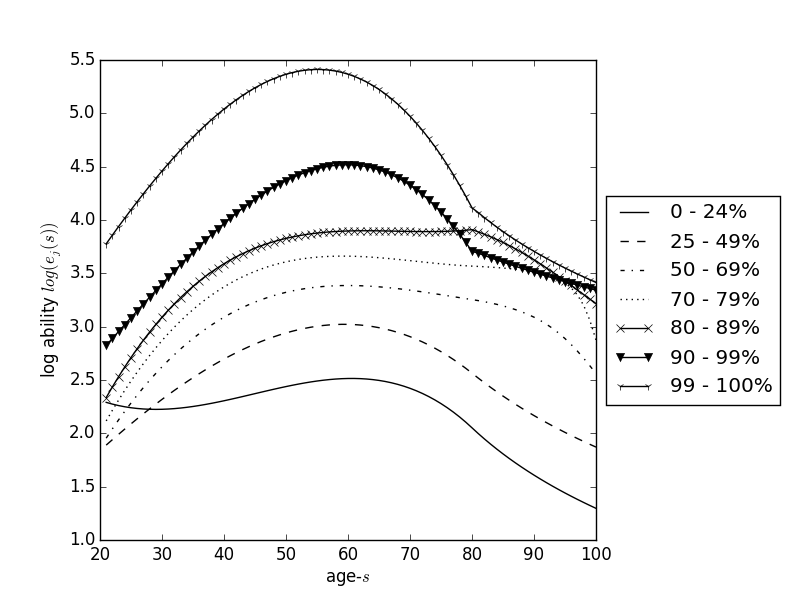
\includegraphics{images/ability_log_2D_no_vline.png}}}
    \end{figure}


  \subsection{Individual problem}\label{SecIndProb}

    Individuals are endowed with a measure of time $\tilde{l}$ in each period $t$, and they choose how much of that time to allocate between labor $n_{j,s,t}$ and leisure $l_{j,s,t}$ in each period. That is, an individual's labor and leisure choice is constrained by his total time endowment, which constraint is identical across all individuals.
    \begin{equation}\label{EqLabConstr}
      n_{j,s,t} + l_{j,s,t} = \tilde{l}
    \end{equation}
    At time $t$, all age-$s$ individuals with ability $e_{j,s}$ know the real wage rate, $w_t$, and know the one-period real net interest rate, $r_t$, on bond holdings, $b_{j,s,t}$, that mature at the beginning of period $t$. They also receive accidental and intentional bequests. They choose how much to consume $c_{j,s,t}$, how much to save for the next period by loaning capital to firms in the form of a one-period bond $b_{j,s+1,t+1}$, and how much to work $n_{j,s,t}$ in order to maximize expected lifetime utility of the following form,
    \begin{equation}\label{EqUtilMax}
      \begin{split}
        &U_{j,s,t} = \sum_{u=0}^{E+S-s}\beta^u\left[\prod_{v=s}^{s+u-1}(1-\rho_v)\right] u\left(c_{j,s+u,t+u},n_{j,s+u,t+u},b_{j,s+u+1,t+u+1}\right) \\
        &\text{and} \quad u\left(c_{j,s,t},n_{j,s,t},b_{j,s+1,t+1}\right) = \frac{\left(c_{j,s,t}\right)^{1-\sigma} - 1}{1-\sigma} ... \\
        &\qquad\qquad + e^{g_y t(1-\sigma)}\chi^n_s\left(b\left[1 - \left(\frac{n_{j,s,t}}{\tilde{l}}\right)^\upsilon\right]^\frac{1}{\upsilon} + k\right) + \rho_s\chi^b_j\frac{\left(b_{j,s+1,t+1}\right)^{1-\sigma} - 1}{1-\sigma} \\
        &\quad\quad\quad\quad\quad\quad\quad\quad\quad\quad\quad\quad\quad\quad\quad\quad\quad\quad\quad\forall j,t\quad\text{and}\:E+1\leq s\leq E+S
      \end{split}
    \end{equation}
    where $\sigma\geq 1$ is the coefficient of relative risk aversion on consumption and on intended (precautionary) bequests, $\beta\in(0,1)$ is the agent's discount factor, and the product term in brackets depreciates the individual's discount factor by the cumulative mortality rate. The disutility of labor term in the period utility function looks nonstandard, but is simply the upper right quadrant of an ellipse that closely approximates the standard CRRA utility of leisure functional form.\footnote{Appendix \ref{AppEllipseUtil} describes how the elliptical function closely matches the more standard utility of leisure of the form $\frac{(\tilde{l}-n_{j,s,t})^{1+\theta}}{1+\theta}$. This elliptical utility function forces an interior solution that automatically respects both the upper and lower bound of labor supply, which greatly simplifies the computation of equilibrium. In addition, the elliptical disutility of labor has a Frisch elasticity that asymptotes to a constant rather than increasing to infinity as it does in the CRRA case. For a more in-depth discussion see \citet{EvanPhillips:2015}} The term $\chi^n_s$ is a constant term that varies by age $s$ influencing the disutility of labor relative to the other arguments in the period utility function,\footnote{\citet{DEMPRW2015} calibrate $\chi^n_s$ and $\chi^b_j$ to match average labor hours by age and some moments of the distribution of wealth.} and $g_y$ is a constant growth rate of labor augmenting technological progress, which we explain in Section \ref{SecFirms}.\footnote{The term with the growth rate $e^{g_y t(1-\sigma)}$ must be included in the period utility function because consumption and bequests will be growing at rate $g_y$ and this term stationarizes the individual Euler equation by making the marginal disutility of labor grow at the same rate as the marginal benefits of consumption and bequests.  This is the same balanced growth technique as that used in \citet{MertensRavn:2011}.}

    The last term in \eqref{EqUtilMax} incorporates a warm-glow bequest motive in which individuals value having savings to bequeath to the next generation in the chance they die before the next period. Including this term is essential to generating the positive wealth levels across the life cycle and across abilities that exist in the data. In addition, the term $\chi^b_j$ is a constant term that varies by lifetime income group $j$ influencing the marginal utility of bequests, $b_{j,s+1,t+1}$ relative to the other arguments in the period utility function. Allowing the $\chi^b_j$ scale parameter on the warm glow bequest motive vary by lifetime income group is critical for matching the distribution of wealth. As was mentioned in Section \ref{SecPopDyn}, individuals in the model have no income uncertainty because each lifetime earnings path $e_{j,s}$ deterministic, model agents thus hold no precautionary savings. Calibrating the $\chi^b_j$ for each income group $j$ captures in a reduced form way some of the characteristics that individual income risk provides.

    The parameter $\sigma\geq 1$ is the coefficient of relative risk aversion on bequests, and the mortality rate $\rho_s$ appropriately discounts the value of this term.\footnote{It is necessary for the coefficient of relative risk aversion $\sigma$ to be the same on both the utility of consumption and the utility of bequests. If not, the resulting Euler equations are not stationarizable.} Note that, because of this bequest motive, individuals in the last period of their lives ($s=S$) will die with positive savings $b>0$. Also note that the CRRA utility of bequests term prohibits negative wealth holdings in the model, but is not a strong restriction since none of the wealth data for the lifetime income group $j$ and age $s$ cohorts is negative except for the lowest quartile.

    The per-period budget constraints for each agent normalized by the price of consumption are the following,
    \begin{equation}\label{EqBC}
      \begin{split}
        &c_{j,s,t} + b_{j,s+1,t+1} \leq \left(1 + r_t\right) b_{j,s,t} + w_t e_{j,s}n_{j,s,t} + \frac{BQ_{j,t}}{\lambda_j\tilde{N}_t} - T_{s,t} \\
        &\qquad\qquad\qquad\text{where}\quad b_{j,E+1,t} = 0\quad\text{for} \quad E+1\leq s \leq E+S \quad \forall j,t
      \end{split}
    \end{equation}
    where $\tilde{N}_t$ is the total working age population at time $t$ defined in \eqref{EqPopWkDef} and $\lambda_j\tilde{N}_t$ is the number of the total working individuals of type $j$ in period $t$. Note that the price of consumption is normalized to one, so $w_t$ is the real wage and $r_t$ is the net real interest rate. The term $BQ_{j,t}$ represents total bequests from individuals in income group $j$ who died at the end of period $t-1$. $T_{s,t}$ is a function representing net taxes paid, which we specify more fully below in equation \eqref{EqNetTaxLiab}.

    Implicit in the period budget constraint \eqref{EqBC} is a strong assumption about the distribution of bequests. We assume that bequests are distributed evenly across all ages to those in the same lifetime income group. It is difficult to precisely calibrate the distribution of bequests from the data, both across income types $j$ and across ages $s$. However, the assumptions about the bequest motive as well as how bequests are distributed are clearly important modeling decisions. Our current specification of bequests is the most persistent, which should make wealth inequality more persistent relative to other bequest specifications.\footnote{Another allocation rule at the opposite extreme would be to equally divide all bequests among all surviving individuals. An intermediate rule would be some kind of distribution of bequests with most going to ones own type and a declining proportion going to the other types.} A large number of papers study the effects of different bequest motives and specifications on the distribution of wealth, though there is no consensus regarding the true bequest transmission process.\footnote{See \citet{DeNardiYang:2014}, \citet{DeNardi:2004}, \citet{Nishiyama:2002}, \citet{Laitner:2001}, \citet{GokhaleEtAl:2000}, \citet{GaleScholz:1994}, \citet{Hurd:1989}, \citet{VentiWise:1988}, \citet{KotlikoffSummers:1981}, and \citet{Wolff:2015}.}

    Because the form of the period utility function in \eqref{EqUtilMax} ensures that $b_{j,s,t}>0$ for all $j$, $s$, and $t$, total bequests will always be positive $BQ_{j,t}>0$ for all $j$ and $t$.
    \begin{equation}\label{EqTotBeq}
      BQ_{j,t+1} = (1+r_{t+1})\lambda_j\left(\sum_{s=E+1}^{E+S}\rho_s\omega_{s,t}b_{j,s+1,t+1}\right) \quad\forall j,t
    \end{equation}
    In addition to each the budget constraint in each period, the utility function \eqref{EqUtilMax} imposes nonnegative consumption through infinite marginal utility, and the elliptical utility of leisure ensures individual labor and leisure must be strictly nonnegative $n_{j,s,t},l_{j,s,t}> 0$. Because individual savings or wealth is always strictly positive, the aggregate capital stock is always positive.\footnote{An alternative would be to allow for individual borrowing as long as an aggregate capital constraint $K_{t}>0$ for all $t$ is satisfied.} An interior solution to the individual's problem \eqref{EqUtilMax} is assured.

    In reality, each household is subject to many different taxes, all of which cannot be modeled in a DGE framework. It is the net tax liability function $T_{s,t}$ that we estimate from the microsimulation model output. This output includes information on all taxes paid in the American tax code. We also assume that every individual also receives an equal lump sum transfer $T^H_{t}$ which is generated from a balanced budget constraint on the government. We represent the net tax liability function as an average effective tax rate times total income.
    \begin{equation}\label{EqNetTaxLiab}
      \begin{split}
        T_{s,t}(x, y) &= \tau_{s,t}(x, y)\bigl(x + y\bigr) - T^H_t \\
        &\text{where}\quad x\equiv \frac{w_t e_{j,s}n_{j,s,t}}{e^{g_y t}} \quad\text{and}\quad y\equiv \frac{r_t b_{j,s,t}}{e^{g_y t}}
      \end{split}
    \end{equation}
    Note that the both the total tax liability function $T_{s,t}(x,y)$ and the average effective tax rate functions $\tau_{s,t}(x,y)$ are functions of stationarized labor income $x$ and capital income $y$, separately. We detail the estimation of the tax functions $\tau_{s,t}(x,y)$ and $T_{s,t}(x,y)$ in Section \ref{SecIntegr}.

    The solution to the lifetime maximization problem \eqref{EqUtilMax} of individual with ability $j$ subject to the per-period budget constraint \eqref{EqBC} and the specification of taxes in \eqref{EqNetTaxLiab} is a system of $2S$ Euler equations. The $S$ static first order conditions for labor supply $n_{j,s,t}$ are the following,
    \begin{equation}\label{EqEulerLabGen}
      \begin{split}
        &(c_{j,s,t})^{-\sigma}\Biggl(w_t e_{j,s} - \frac{\partial T_{s,t}}{\partial n_{j,s,t}}\Biggr) = e^{g_y t(1-\sigma)}\chi^n_{s}\biggl(\frac{b}{\tilde{l}}\biggr)\biggl(\frac{n_{j,s,t}}{\tilde{l}}\biggr)^{v-1}\Biggl[1 - \biggl(\frac{n_{j,s,t}}{\tilde{l}}\biggr)^\upsilon\Biggr]^{\frac{1-v}{v}} \\
        &\qquad\qquad\qquad\qquad\qquad\qquad\qquad\qquad\qquad\forall j,t, \quad\text{and}\quad E+1\leq s\leq E+S \\
        &\qquad\text{where}\quad c_{j,s,t} = \left(1 + r_t\right) b_{j,s,t} + w_t e_{j,s}n_{j,s,t} + \frac{BQ_{j,t}}{\lambda_j\tilde{N}_t} - b_{j,s+1,t+1} - T_{s,t} \\
        &\qquad\text{and}\quad b_{j,E+1,t} = 0 \quad\forall j,t
      \end{split}
    \end{equation}
    where the marginal tax rate with respect to labor supply $\frac{\partial T_{s,t}}{\partial n_{j,s,t}}$ is described in equation \ref{EqMTRx}.\footnote{We also have to use a parameter $H$ that multiplies the model labor income and the model capital income in the tax function in order to match their levels to the corresponding average levels in the microsimulation model data.}

    An individual also has $S-1$ dynamic Euler equations that govern his saving decisions, $b_{j,s+1,t+1}$, with the included precautionary bequest saving in case of unexpected death. These are given by:
    \begin{equation}\label{EqEulerSavGen}
      \begin{split}
        &(c_{j,s,t})^{-\sigma} = \rho_s\chi^b_j\bigl(b_{j,s+1,t+1}\bigr)^{-\sigma} + \beta(1-\rho_s)(c_{j,s+1,t+1})^{-\sigma}\Biggl[(1 + r_{t+1}) - \frac{\partial T_{j,s+1,t+1}}{\partial b_{j,s+1,t+1}}\Biggr] \\
        &\qquad\qquad\qquad\qquad\qquad\qquad\qquad\qquad\forall j,t,\quad\text{and}\quad E+1\leq s \leq E+S-1 \\
        &\qquad\text{where}\quad \frac{\partial T_{j,s+1,t+1}}{\partial b_{j,s+1,t+1}} = ...\\
        &\qquad\qquad r_{t+1}\Biggl(\tau^I(F\hat{a}_{j,s+1,t+1}) + \frac{F\hat{a}_{j,s+1,t+1}CD\left[2A(F\hat{a}_{j,s+1,t+1}) + B\right]}{\left[A(F\hat{a}_{j,s+1,t+1})^2 + B(F\hat{a}_{j,s+1,t+1}) + C\right]^2}\Biggr) ... \\
        &\qquad\qquad + \tau^W(\hat{b}_{j,s+1,t+1}) + \frac{\hat{b}_{j,s+1,t+1}PHM}{\left(H\hat{b}_{j,s+1,t+1} + M\right)^2}
      \end{split}
    \end{equation}
    The parameters $P$, $H$, and $M$ characterize the progressive wealth tax function $\tau^W(\hat{b}) = P\frac{H\hat{b}}{H\hat{b}+M}$. In the baseline, the wealth tax is zero.\footnote{In the wealth tax experiment, the parameters are calibrated so that the tax rate on average wealth in the steady state is one percent, the rate on the highest steady-state wealth is two percent, and the rate on the highest steady-state wealth is 2.5 percent.} Lastly, Each individual also has one static first order condition for the last period of life $s=E+S$, which governs how much to bequeath to the following generation given that the individual will die with certainty.  This condition is:
    \begin{equation}\label{EqEulerSavEpS}
      (c_{j,E+S,t})^{-\sigma} = \chi^b_j(b_{j,E+S+1,t+1})^{-\sigma} \quad\forall j,t
    \end{equation}

    Define $\bm{\hat{\Gamma}}_t$ as the distribution of stationary individual savings across individuals at time $t$, including the intentional bequests of the oldest cohort.
    \begin{equation}\label{EqSavDist}
      \bm{\hat{\Gamma}}_t \equiv \Bigl\{\bigl\{\hat{b}_{j,s,t}\bigr\}_{j=1}^J\Bigr\}_{s=E+2}^{E+S+1} \quad\forall t
    \end{equation}
    As will be shown in Section \ref{SecMCEqlbm}, the state in every period $t$ for the entire equilibrium system described in the stationary, non-steady-state equilibrium characterized in Definition \ref{DefEquilNonSS} is the stationary distribution of individual savings $\bm{\hat{\Gamma}}_t$ from \eqref{EqSavDist}. Because individuals must forecast wages, interest rates, and aggregate bequests received in every period in order to solve their optimal decisions and because each of those future variables depends on the entire distribution of savings in the future, we must assume some individual beliefs about how the entire distribution will evolve over time. Let general beliefs about the future distribution of capital in period $t+u$ be characterized by the operator $\Omega(\cdot)$ such that:
    \begin{equation}\label{EqBeliefs}
      \bm{\hat{\Gamma}^e_{t+u}} = \Omega^u\left(\bm{\hat{\Gamma}_t}\right) \quad \forall t, \quad u\geq 1
    \end{equation}
    where the $e$ superscript signifies that $\hat{\Gamma}^e_{t+u}$ is the expected distribution of wealth at time $t+u$ based on general beliefs $\Omega(\cdot)$ that are not constrained to be correct.\footnote{In Section \ref{SecMCEqlbm} we will assume that beliefs are correct (rational expectations) for the stationary non-steady-state equilibrium in Definition \ref{DefEquilNonSS}.}


  \subsection{Firm problem}\label{SecFirms}

    A unit measure of identical, perfectly competitive firms exist in the economy. The representative firm is characterized by the following Cobb-Douglas production technology,
    \begin{equation}\label{EqCobbDougProd}
       Y_t = Z K_t^\alpha\left(e^{g_y t}L_t\right)^{1-\alpha} \quad \forall t
    \end{equation}
    where $Z$ is the measure of total factor productivity, $\alpha\in(0,1)$ is the capital share of income, $g_y$ is the constant growth rate of labor augmenting technological change, and $L_t$ is aggregate labor measured in efficiency units. The firm uses this technology to produce a homogeneous output which is consumed by individuals and used in firm investment.  The interest rate $r_t$ paid to the owners of capital is the real interest rate net of depreciation. The real wage is $w_t$.  The real profit function of the firm is the following.
    \begin{equation}\label{EqFirmProfit}
       \text{Real Profits} = Z K_t^\alpha\left(e^{g_y t}L_t\right)^{1-\alpha} - (r_t + \delta)K_t - w_t L_t
    \end{equation}
    As in the individual budget constraint \eqref{EqBC}, note that the price output has been normalized to one.

    Profit maximization results in the real wage, $w_t$, and the real rental rate of capital $r_t$ being determined by the marginal products of labor and capital, respectively:
    \begin{align}
       w_t &= (1-\alpha)\frac{Y_t}{L_t} \quad \forall t \label{EqFOCwage}\\
       r_t &= \alpha\frac{Y_t}{K_t} - \delta \quad\:\:\: \forall t \label{EqFOCrate}
    \end{align}


  \subsection{Government fiscal policy}\label{SecGovt}

    The government is represented by a balanced budget constraint. The government collects taxes ($\tau_{s,t}(x,y)(x+y)$) from all individuals and divides total revenues equally among individuals in the economy to determine the lump-sum transfer.
    \begin{equation}\label{EqGovtBC}
      T^H_t = \frac{1}{\tilde N_t} \sum_s \sum_j \omega_{s,t}\lambda_j\tau_{s,t}(w_t e_{j,s}n_{j,s,t}, r_t b_{j,s,t})\bigl(w_t e_{j,s}n_{j,s,t} + r_t b_{j,s,t}\bigr)
    \end{equation}

    Lump sum transfers have an impact on the distribution of income and wealth. However, if one constrains policy experiments to have the same steady-state revenue impact, the changes in inequality in economic outcomes due to changes in government transfers is equivalent in each policy experiment in the steady-state.


  \subsection{Market clearing and stationary equilibrium}\label{SecMCEqlbm}

    Labor market clearing requires that aggregate labor demand $L_t$ measured in efficiency units equal the sum of individual efficiency labor supplied $e_{j,s}n_{j,s,t}$. Capital market clearing requires that aggregate capital demand $K_t$ equal the sum of capital investment by individuals $b_{j,s,t}$. Aggregate consumption $C_t$ is defined as the sum of all individual consumptions, and aggregate investment is defined by the resource constraint $Y_t = C_t + I_t$ as shown in \eqref{EqMktClrGoods}. That is, the following conditions must hold:
    \begin{align}
      L_t &= \sum_{s=E+1}^{E+S}\sum_{j=1}^{J} \omega_{s,t}\lambda_j e_{j,s}n_{j,s,t} \quad \forall t \label{EqMktClrLab} \\
      K_t &= \sum_{s=E+2}^{E+S+1}\sum_{j=1}^{J}\omega_{s-1,t-1}\lambda_j b_{j,s,t}  \quad \forall t \label{EqMktClrCap} \\
      \begin{split}
        Y_t &= C_t + K_{t+1} - (1-\delta)K_t \quad\forall t \\
        &\quad\text{where}\quad C_t \equiv \sum_{s=E+1}^{E+S}\sum_{j=1}^{J}\omega_{s,t}\lambda_j c_{j,s,t}
      \end{split} \label{EqMktClrGoods}
    \end{align}

    The usual definition of equilibrium would be allocations and prices such that individuals optimize \eqref{EqEulerLabGen}, \eqref{EqEulerSavGen}, and \eqref{EqEulerSavEpS}, firms optimize \eqref{EqFOCwage} and \eqref{EqFOCrate}, and markets clear \eqref{EqMktClrLab} and \eqref{EqMktClrCap}. However, the variables in the equations characterizing the equilibrium are potentially non-stationary due to the growth rate in the total population $g_{n,t}$ each period coming from the cohort growth rates in \eqref{EqPopLawofmotion} and from the deterministic growth rate of labor augmenting technological change $g_y$ in \eqref{EqCobbDougProd}.

    \begin{table}[htbp] \centering \captionsetup{width=3.3in}
    \caption{\label{TabStatVars}\textbf{Stationary variable definitions}}
      \begin{threeparttable}
      \begin{tabular}{>{\small}c >{\small}c >{\small}c |>{\small}c}
        \hline\hline
        \multicolumn{3}{c}{Sources of growth} & Not \\
        & & & \\[-4mm]
        $e^{g_y t}$ & $\tilde{N}_t$ & $e^{g_y t}\tilde{N}_t$ & growing\tnote{a} \\
        \hline
        & & \\[-4mm]
        $\hat{c}_{j,s,t}\equiv\frac{c_{j,s,t}}{e^{g_y t}}$ & $\hat{\omega}_{s,t}\equiv\frac{\omega_{s,t}}{\tilde{N}_t}$ & $\hat{Y}_t\equiv\frac{Y_t}{e^{g_y t}\tilde{N}_t}$ & $n_{j,s,t}$ \\[2mm]
        $\hat{b}_{j,s,t}\equiv\frac{b_{j,s,t}}{e^{g_y t}}$ & $\hat{L}_t\equiv\frac{L_t}{\tilde{N}_t}$ & $\hat{K}_t\equiv\frac{K_t}{e^{g_y t}\tilde{N}_t}$ & $r_t$ \\[2mm]
        $\hat{w}_t\equiv\frac{w_t}{e^{g_y t}}$ &  & $\hat{BQ}_{j,t}\equiv\frac{BQ_{j,t}}{e^{g_y t}\tilde{N}_t}$ &  \\[2mm]
        $\hat{y}_{j,s,t}\equiv\frac{y_{j,s,t}}{e^{g_y t}}$ &  &  &  \\[2mm]
        $\hat{T}_{j,s,t}\equiv\frac{T_{j,s,t}}{e^{g_y t}}$ &  &  &  \\[2mm]
        \hline\hline
      \end{tabular}
      \begin{tablenotes}
        \scriptsize{\item[a]The interest rate $r_t$ in \eqref{EqFOCrate} is already stationary because $Y_t$ and $K_t$ grow at the same rate. Individual labor supply $n_{j,s,t}$ is stationary.}
      \end{tablenotes}
      \end{threeparttable}
    \end{table}

    Table \ref{TabStatVars} characterizes the stationary versions of the variables of the model in terms of the variables that grow because of labor augmenting technological change, population growth, both, or none. With the definitions in Table \ref{TabStatVars}, it can be shown that the equations  characterizing the equilibrium can be written in stationary form in the following way. The static and intertemporal first-order conditions from the individual's optimization problem corresponding to \eqref{EqEulerLabGen}, \eqref{EqEulerSavGen}, and \eqref{EqEulerSavEpS} are the following:

    \begin{equation}\label{EqEulerLabStat}
      \begin{split}
        &(\hat{c}_{j,s,t})^{-\sigma}\Biggl(\hat{w}_t e_{j,s} - \frac{\partial\hat{T}_{j,s,t}}{\partial n_{j,s,t}}\Biggr) = \chi^n_{s}\biggl(\frac{b}{\tilde{l}}\biggr)\biggl(\frac{n_{j,s,t}}{\tilde{l}}\biggr)^{\upsilon-1}\Biggl[1 - \biggl(\frac{n_{j,s,t}}{\tilde{l}}\biggr)^\upsilon\Biggr]^{\frac{1-\upsilon}{\upsilon}} \\
        &\qquad\qquad\qquad\qquad\qquad\qquad\qquad\qquad\forall j,t, \quad\text{and}\quad E+1\leq s\leq E+S \\
        &\qquad\text{where}\quad \hat{c}_{j,s,t} = \left(1 + r_t\right)\hat{b}_{j,s,t} + \hat{w}_t e_{j,s}n_{j,s,t} + \frac{\hat{BQ}_{j,t}}{\lambda_j} - e^{g_y}\hat{b}_{j,s+1,t+1} - \hat{T}_{j,s,t} \\
        &\qquad\text{and}\quad \frac{\partial \hat{T}_{j,s,t}}{\partial n_{j,s,t}} = \hat{w}_t e_{j,s}\biggl[\tau^I\bigl(F\hat{a}_{j,s,t}\bigr) + \frac{F\hat{a}_{j,s,t}CD\bigl[2A(F\hat{a}_{j,s,t})+B\bigr]}{\bigl[A(F\hat{a}_{j,s,t})^2+B(F \hat{a}_{j,s,t})+C\bigr]^2} + \tau^P\Biggr] \\
        &\qquad\text{and}\quad \hat{b}_{j,E+1,t} = 0 \quad\forall j,t
      \end{split}
    \end{equation}

    \begin{equation}\label{EqEulerSavStat}
      \begin{split}
        &(\hat{c}_{j,s,t})^{-\sigma} = ... \\
        &e^{-g_y\sigma}\Biggl(\rho_s\chi^b_j \bigl(\hat{b}_{j,s+1,t+1}\bigr)^{-\sigma} + \beta(1-\rho_s)(\hat{c}_{j,s+1,t+1})^{-\sigma}\Biggl[(1 + r_{t+1}) - \frac{\partial T_{j,s+1,t+1}}{\partial b_{j,s+1,t+1}}\Biggr]\Biggr) \\
        &\qquad\qquad\qquad\qquad\qquad\qquad\qquad\qquad\forall j,t,\quad\text{and}\quad E+1\leq s \leq E+S-1 \\
        &\qquad\text{where}\quad \frac{\partial T_{j,s+1,t+1}}{\partial b_{j,s+1,t+1}} = ...\\
        &\qquad\qquad r_{t+1}\Biggl(\tau^I(F\hat{a}_{j,s+1,t+1}) + \frac{F\hat{a}_{j,s+1,t+1}CD\left[2A(F\hat{a}_{j,s+1,t+1}) + B\right]}{\left[A(F\hat{a}_{j,s+1,t+1})^2 + B(F\hat{a}_{j,s+1,t+1}) + C\right]^2}\Biggr) ... \\
        &\qquad\qquad + \tau^W(\hat{b}_{j,s+1,t+1}) + \frac{\hat{b}_{j,s+1,t+1}PHM}{\left(H\hat{b}_{j,s+1,t+1} + M\right)^2}
      \end{split}
    \end{equation}

    \begin{equation}\label{EqEulerSavEpSstat}
      (\hat{c}_{j,E+S,t})^{-\sigma} = \chi^b_j e^{-g_y\sigma}(\hat{b}_{j,E+S+1,t+1})^{-\sigma} \quad\forall j,t
    \end{equation}

    The stationary firm first order conditions for optimal labor and capital demand corresponding to \eqref{EqFOCwage} and \eqref{EqFOCrate} are the following.
    \begin{equation}\label{EqFOCwageStat}
       \hat{w}_t = (1-\alpha)\frac{\hat{Y}_t}{\hat{L}_t} \quad \forall t
    \end{equation}
    \begin{equation}\tag{\ref{EqFOCrate}}
       r_t = \alpha\frac{\hat{Y}_t}{\hat{K}_t} - \delta = \alpha\frac{Y_t}{K_t} - \delta \quad \forall t
    \end{equation}
    And the two stationary market clearing conditions corresponding to \eqref{EqMktClrLab} and \eqref{EqMktClrCap}---with the goods market clearing by Walras' Law---are the following.
    \begin{align}
      \hat{L}_t &= \sum_{s=E+1}^{E+S}\sum_{j=1}^{J} \hat{\omega}_{s,t}\lambda_j e_{j,s}n_{j,s,t} \quad \forall t \label{EqMktClrLabStat} \\
      \hat{K}_t &= \frac{1}{1 + \tilde{g}_{n,t}}\left(\sum_{s=E+2}^{E+S+1}\sum_{j=1}^{J}\hat{\omega}_{s-1,t-1}\lambda_j \hat{b}_{j,s,t}\right) \quad \forall t \label{EqMktClrCapStat}
    \end{align}
    where $\tilde{g}_{n,t}$ is the growth rate in the working age population between periods $t-1$ and $t$ described in \eqref{EqPopWkGrowth}. It is also important to note the stationary version of the characterization of total bequests $BQ_{j,t+1}$ from \eqref{EqTotBeq} and for the government budget constraint in \eqref{EqGovtBC}.
    \begin{equation}\label{EqTotBeqStat}
      \hat{BQ}_{j,t+1} = \frac{(1+r_{t+1})\lambda_j}{1+\tilde{g}_{n,t}}\left(\sum_{s=E+1}^{E+S}\rho_s\hat{\omega}_{s,t}\hat{b}_{j,s+1,t+1}\right) \quad\forall j,t
    \end{equation}
    \begin{equation}\label{EqGovtBCstat}
      \hat{T}^H_t = \sum_s \sum_j \hat{\omega}_{s,t}\lambda_j\left(\hat{T}^I_{j,s,t} + \hat{T}^P_{j,s,t} + \hat{T}^{BQ}_{j,s,t} + \hat{T}^W_{j,s,t}\right)
    \end{equation}

    We can now define the stationary steady-state equilibrium for this economy in the following way.

    \vspace{7mm}
    \end{spacing}
    \hrule
    \begin{definition}[\textbf{Stationary steady-state equilibrium}]\label{DefEquilSS}
      A non-autarkic stationary steady-state equilibrium in the overlapping generations model with $S$-period lived agents and heterogeneous ability $e_{j,s}$ is defined as constant allocations $n_{j,s,t}=\bar{n}_{j,s}$ and $\hat{b}_{j,s+1,t+1}=\bar{b}_{j,s+1}$ and constant prices $\hat{w}_t=\bar{w}$ and $r_t=\bar{r}$ for all $j$, $s$, and $t$ such that the following conditions hold:
       \begin{enumerate}
          \item individuals optimize according to \eqref{EqEulerLabStat}, \eqref{EqEulerSavStat}, and \eqref{EqEulerSavEpSstat},
          \item Firms optimize according to \eqref{EqFOCwageStat} and \eqref{EqFOCrate},
          \item Markets clear according to \eqref{EqMktClrLabStat} and \eqref{EqMktClrCapStat}, and
          \item The population has reached its stationary steady state distribution $\bar{\omega}_s$ for all ages $s$, characterized in Appendix \ref{AppPopGrowth}.
       \end{enumerate}
    \end{definition}
    \hrule
    \begin{spacing}{1.5}
    \vspace{10mm}

    The steady-state equilibrium is characterized by the system of $2JS$ equations and $2JS$ unknowns $\bar{n}_{j,s}$ and $\bar{b}_{j,s+1}$. Appendix \ref{AppSSsolve} details how to solve for the steady-state equilibrium. Because our qualitative results and conclusions are unchanged across the equilibrium time path of the economy from the baseline steady state to the new steady state after the policy change, we confine our definition of the non-steady-state equilibrium and its computational solution to Appendix \ref{AppNonSSsolve}.\footnote{We can provide equilibrium time path solutions for each policy experiment upon request.}


  \subsection{Calibration}\label{SecCalib}

    Table \ref{TabExogVars} shows the calibrated values for the exogenous variables and parameters. The values of these parameters come from \citet{DEMPRS2015}.

    \begin{table}[htbp] \centering \captionsetup{width=4.7in}
    \caption{\label{TabExogVars}\textbf{List of exogenous variables and baseline calibration values}}
      \begin{threeparttable}
      \begin{tabular}{>{\footnotesize}c |>{\footnotesize}l |>{\footnotesize}c}
        \hline\hline
        Symbol & \quad\quad\quad\quad Description & Value \\
        \hline
        $\bm{\hat{\Gamma}}_1$ & Initial distribution of savings & $\bm{\bar{\Gamma}}$ \\
        $N_0$ & Initial population & 1 \\
        $\{\omega_{s,0}\}_{s=1}^S$ & Initial population by age & (see App. \ref{AppPopGrowth}) \\
        $\{f_s\}_{s=1}^S$ & Fertility rates by age & (see App. \ref{AppPopGrowth}) \\
        $\{i_s\}_{s=1}^S$ & Immigration rates by age & (see App. \ref{AppPopGrowth}) \\
        $\{\rho_s\}_{s=1}^S$ & Mortality rates by age & (see App. \ref{AppPopGrowth}) \\
        $\{e_{j,s}\}_{j,s=1}^{J,S}$ & Deterministic ability process & (see App. \ref{AppAbilCalib}) \\
        $\{\lambda_j\}_{j=1}^J$ & Lifetime income group percentages & (see App. \ref{AppAbilCalib}) \\
        $J$ & Number of lifetime income groups & 7 \\
        $S$ & Maximum periods in economically active & 80 \\[-2mm]
        &\quad individual life & \\
        $E$ & Number of periods of youth economically & $\text{round}\left(\frac{S}{4}\right)$ \\[-2mm]
        & \quad outside the model & \\
        $R$ & Retirement age (period) & $\text{round}\left(\frac{9}{16}S\right)$ \\
        \hline
        $\tilde{l}$ & Maximum hours of labor supply & 1 \\
        $\beta$ & Discount factor & $(0.96)^\frac{80}{S}$ \\
        $\sigma$ & Coefficient of constant relative risk aversion & 3 \\
        $b$ & Scale parameter in utility of leisure & (see App. \ref{AppEllipseUtil}) \\
        $\upsilon$ & Shape parameter in utility of leisure & (see App. \ref{AppEllipseUtil}) \\
        $k$ & constant parameter in utility of leisure & (see App. \ref{AppEllipseUtil}) \\
        $\chi^n_s$ & Disutility of labor level parameters & (see Sec. \ref{sec:calib}) \\
        $\chi^b_j$ & Utility of bequests level parameters &  $[9.264 \times 10^{-5}, 118,648.915]$ \\
        \hline
        $Z$ & Level parameter in production function & 1 \\
        $\alpha$ & Capital share of income & 0.35 \\
        $\delta$ & Capital depreciation rate & $1-(1-0.05)^\frac{80}{S}$ \\
        $g_y$ & Growth rate of labor augmenting & $(1+0.03)^\frac{80}{S}-1$ \\[-2mm]
        & \quad technological progress & \\
%        \hline
%        $A$ & Coefficient on squared term in $\tau^I(\cdot)$ & (see App. \ref{AppIncTaxRate}) \\
%        $B$ & Coefficient on linear term in $\tau^I(\cdot)$ & (see App. \ref{AppIncTaxRate}) \\
%        $C$ & Constant coefficient in $\tau^I(\cdot)$ & (see App. \ref{AppIncTaxRate}) \\
%        $D$ & Level parameter for $\tau^I(\cdot)$ & (see App. \ref{AppIncTaxRate}) \\
%        $F$ & Income factor for $\tau^I(\cdot)$ & (see App. \ref{AppIncTaxRate}) \\
%        $\tau^P$ & Payroll tax rate & 0.15 \\
%        $\{\theta^j\}_{j=1}^J$ & Replacement rate by average income & (see App. \ref{AppReplRate}) \\
%        $\tau^{BQ}$ & Bequest (estate) tax rate & 0 \\
%        $P$ & Level parameter for $\tau^W(\cdot)$ & 0 \\
%        $H$ & Coefficient on linear term in $\tau^W(\cdot)$ & 1 \\
%        $M$ & Constant coefficient in $\tau^W(\cdot)$ & 1 \\
        \hline
        $T$ & Number of periods to steady state & 160 \\
        $\nu$ & Dampening parameter for TPI & 0.2 \\
        \hline\hline
      \end{tabular}
      % \begin{tablenotes}
      %   \scriptsize{\item[]Note: Maybe put sources here.}
      % \end{tablenotes}
      \end{threeparttable}
    \end{table}

   Note that the scale parameter $\chi^n_s$ takes on 80 values (one for each model age) that increase with age, representing an increasing disutility of labor that is not modeled anywhere else in the utility function. An hour of labor for an older person becomes more costly due to biological reasons related to aging. Such a parametrization helps to fit fact that hours worked decline much more sharply later in life than do hourly earnings.

   Heterogeneity in the scale parameter multiplying useful in having the model generate a distribution of wealth similar to that observed in the data.  Note that without such heterogeneity in this parameter, individuals at the high end of the earnings distribution in our model would not save as much as their real world counterparts given the deterministic earnings process in our model. They have no precautionary savings motive, only the warm-glow bequest motive for savings.  One can view the assumption of heterogeneous utility weights as not just variation in preference across households, but also as reflecting differences in family size, expectations of income growth, or other variations that are not explicitly modeled here.  We thus allow  $\{\chi^b_j\}_{j=1}^7$ to take on seven values, one for each lifetime income group.


%    \begin{figure}[htb]\centering \captionsetup{width=4.0in}
%      \caption{\label{fig:chi_n}\textbf{Calibrated values of $\chi^n_s$}}
%      \fbox{\resizebox{4.0in}{3.0in}{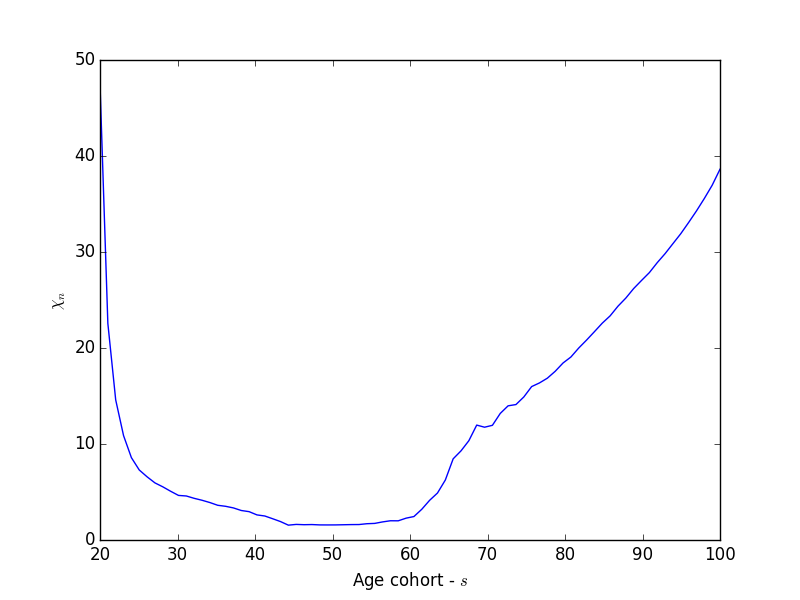
\includegraphics{images/chi_n.png}}}
%    \end{figure}
%
%    \begin{figure}[htb]\centering \captionsetup{width=4.0in}
%      \caption{\label{fig:labor_model_data}\textbf{Life-cycle Average Labor Supply: Model vs. Data}}
%      \fbox{\resizebox{4.0in}{3.0in}{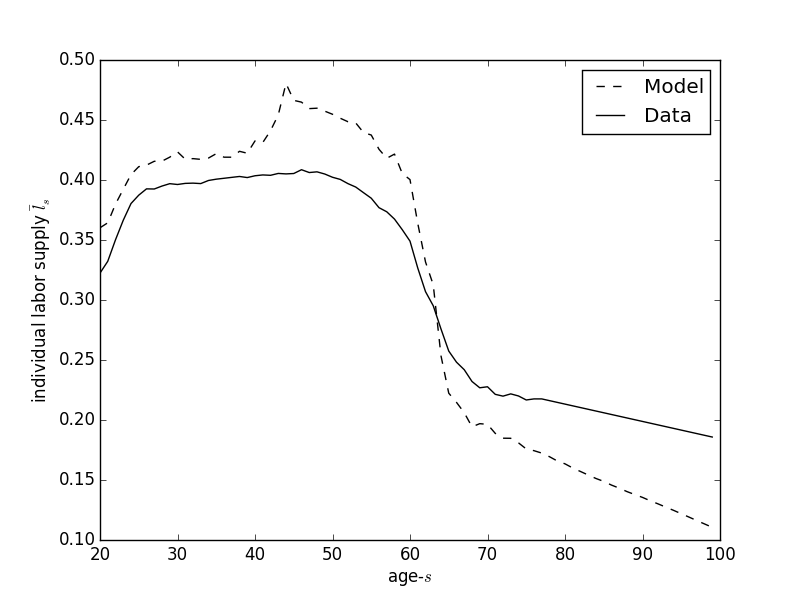
\includegraphics{images/labor_dist_comparison.png}}}
%    \end{figure}
%
%    \begin{figure}[htb]\centering \captionsetup{width=4.0in}
%      \caption{\label{fig:labor_dist_data_fit}\textbf{Labor Distribution from Data, with extrapolation}}
%      \fbox{\resizebox{4.0in}{3.0in}{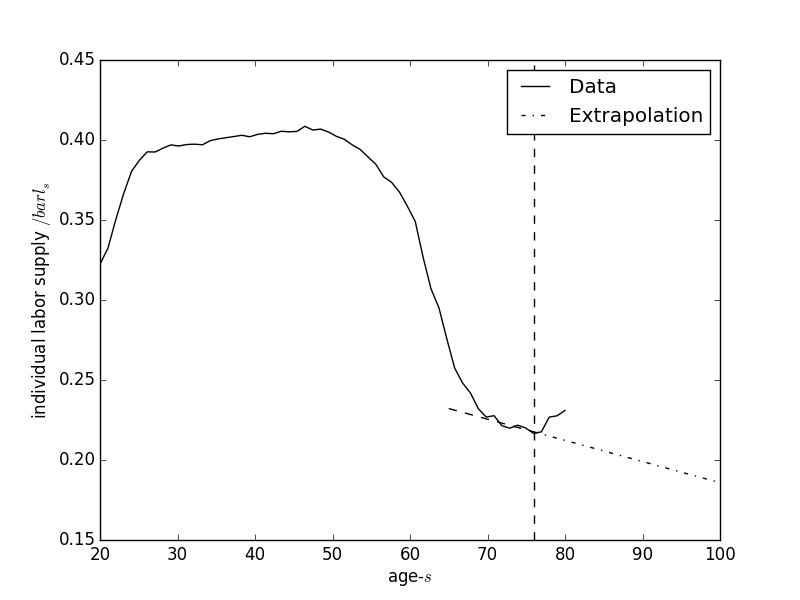
\includegraphics{images/labor_dist_data_withfit.png}}}
%    \end{figure}
%
%    \begin{figure}[htbp]\centering \captionsetup{width=4.0in}
%      \caption{\label{fig:wealth_model_data}\textbf{Wealth over the life-cycle by age for each lifetime earnings group: Model vs. Data}}
%      \fbox{\resizebox{4.0in}{5.5in}{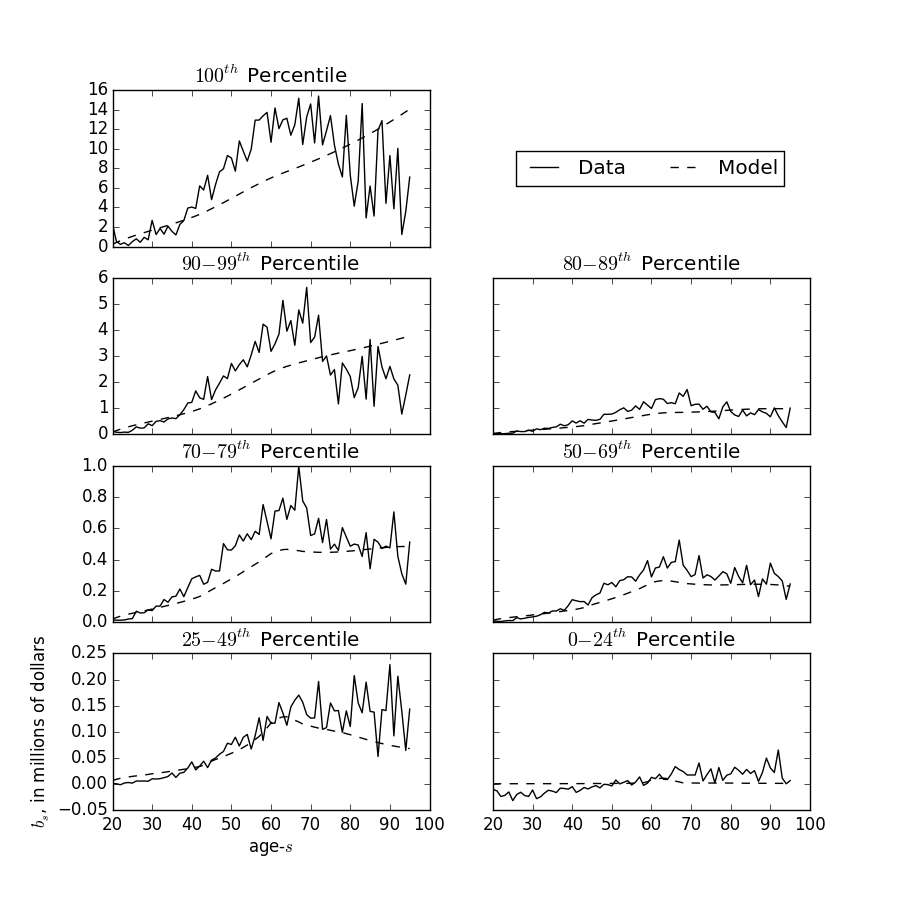
\includegraphics{images/wealth_dist_comparison.png}}}
%    \end{figure}

    \clearpage

    % \begin{table}[htbp] \centering \captionsetup{width=4.5in}
    %   \caption{\label{TabWealthMoms}\textbf{Comparison of average wealth holdings moments (in dollars) between the model and data, by age and income group}}
    %     \begin{threeparttable}
    %     \begin{tabular}{>{\footnotesize}l |>{\footnotesize}l |>{\footnotesize}c |>{\footnotesize}c |>{\footnotesize}c >{\footnotesize}c >{\footnotesize}c}
    %       \hline\hline
    %       \multicolumn{1}{c}{\footnotesize{Income Group}} & \multicolumn{1}{c}{\footnotesize{}} & \multicolumn{1}{c}{\footnotesize{Average wealth}} & \multicolumn{1}{c}{\footnotesize{Average wealth}} &  \multicolumn{1}{c}{\footnotesize{Percent}}\\
    %       \multicolumn{1}{c}{\footnotesize{(percentile)}}& \multicolumn{1}{c}{\footnotesize{Age Group}} & \multicolumn{1}{c}{\footnotesize{model steady state}} & \multicolumn{1}{c}{\footnotesize{Data}} & \multicolumn{1}{c}{\footnotesize{Difference}}\\
    %       \hline
    %       0\%-24\%   & ages 21 to 45 & 432.35 & -16,011.93\tnote{a} & 102.7 \%\\
    %                  & ages 45 to 65 & 3,347.79 & 5,916.55 & -43.4\% \\
    %       \hline
    %       25\%-49\%  & ages 21 to 45 & 21,090.65 & 17,155.31 &  22.9\% \\
    %                  & ages 45 to 65 & 81,229.52 & 100,570.01 &  -19.2\% \\
    %       \hline
    %       50\%-69\%  & ages 21 to 45 & 51,502.14 & 66,589.05 &  -22.7\% \\
    %                  & ages 45 to 65 & 188,324.24 & 297,851.75 &  -37.8\% \\
    %       \hline
    %       70\%-79\%  & ages 21 to 45 & 94,511.89 & 146,347.66 &  -35.4\% \\
    %                  & ages 45 to 65 & 338,299.41 & 577,941.17 &  -41.5\% \\
    %       \hline
    %       80\%-89\%  & ages 21 to 45 & 180,240.48 & 261,039.27 &  -31.0\% \\
    %                  & ages 45 to 65 & 613,371.04 & 1,002,995.73 &  -38.8\% \\
    %       \hline
    %       90\%-98\%  & ages 21 to 45 & 558,903.46 & 720,473.78 &  -22.4\% \\
    %                  & ages 45 to 65 & 1,870,106.49 & 3,178,335.54 &  -41.2\% \\
    %       \hline
    %       99\%-100\% & ages 21 to 45 & 1,856,446.62 & 2,363,198.97 &  -21.4\% \\
    %                  & ages 45 to 65 & 5,748,935.34 & 10,803,634.69 &  -46.8\% \\
    %       \hline
    %       \hline\hline
    %     \end{tabular}
    %     \begin{tablenotes}
    %       \scriptsize{\item[a]Because average wealth holdings for the bottom quartile of wealth holders age 21 to 45 is the only data category with a negative average wealth, we calibrated our parameters to match a positive number very close to zero (\$ 500). Otherwise, our minimization routine would search indefinitely for a solution. The model cannot generate negative wealth.}
    %     \end{tablenotes}
    %     \end{threeparttable}
    % \end{table}

%        The average labor hours data from Figures \ref{fig:labor_model_data} and \ref{fig:labor_dist_data_fit} come from the Current Population Survey (CPS) March Supplement from 1992 to 2013. We determined hours worked in a year by the average hours worked per week in the last year and the number of weeks worked in the last year. We then compute mean hours worked by year of age using population weights. CPS on those near age 80 are noisy, thus we smooth the hours worked data for these year in the following way. We linearly fit the hours works fro ages 76 to 100 using the slope from hours worked for ages 60 to 76. For the average wealth by age and income group in Figure \ref{fig:wealth_model_data}, we use the 2007, 2010, and 2013 Survey of Consumer Finances and obtain the distribution of total net worth by age using population weights.

    %%% note that the SCF wealth data are in 2013$ and the wage profiles for ability are in 2005$. This maybe problematic if we are calibrating using the levels of wealth. If we use shares, we are ok.

%    Figure \ref{FigLabSS} shows the stationary steady-state distribution of individual labor supply $\bar{n}_{j,s}$ and Figure \ref{FigConsSS} shows the steady-state distribution of consumption $\bar{c}_{j,s}$ for the baseline calibration of the model described in Table \ref{TabExogVars}. Notice from Figure \ref{FigConsSS} the hump-shaped pattern of consumption over the life cycle for each ability type, which is consistent with consumption data.
%
%    \begin{figure}[htb]\centering \captionsetup{width=4.0in}
%      \caption{\label{FigLabSS}\textbf{Stationary steady-state distribution of individual labor supply $\bar{n}_{j,s}$ for $S=80$ and $J=7$} from baseline model}
%      \fbox{\resizebox{4.0in}{3.0in}{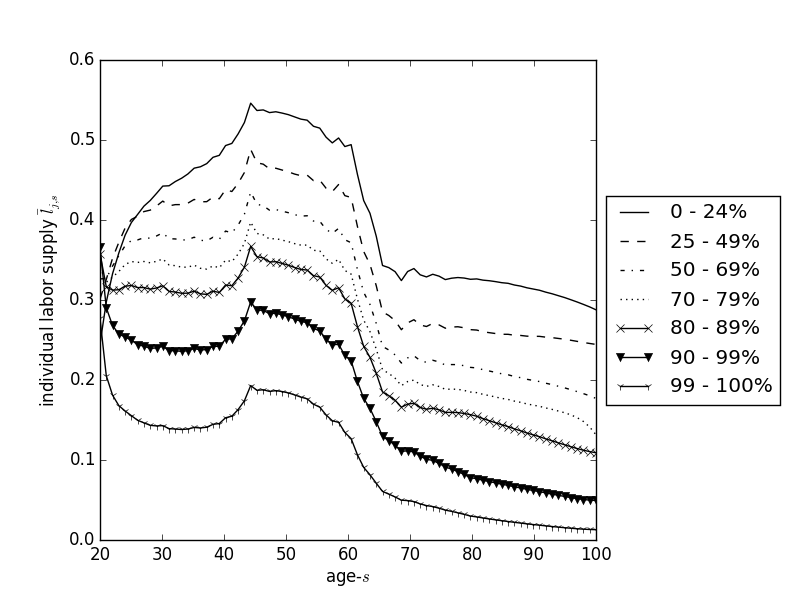
\includegraphics{images/labor_dist_2D.png}}}
%    \end{figure}
%
%    \begin{figure}[htb]\centering \captionsetup{width=4.0in}
%      \caption{\label{FigConsSS}\textbf{Stationary steady-state distribution of consumption $\bar{c}_{j,s}$ for $S=80$ and $J=7$ in baseline model}}
%      \fbox{\resizebox{4.0in}{3.0in}{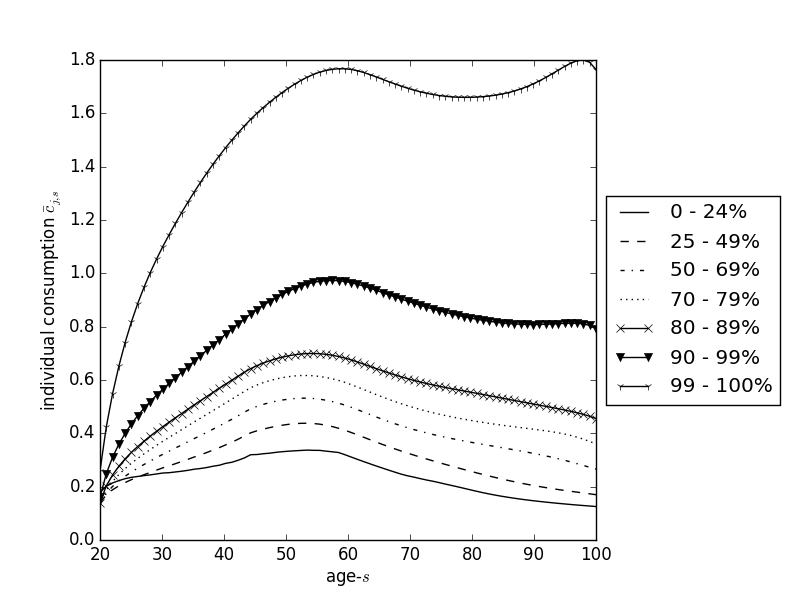
\includegraphics{images/consumption_2D.png}}}
%    \end{figure}

    \FloatBarrier


\section{Integration of Microsimulation Model with DGE Model}\label{SecIntegr}

 The interface between the microsimulation and DGE model will take place through the tax function, $T_{j,s,t}$, and in particular the income and payroll tax functions, $T^I_{j,s,t} + T^P_{j,s,t}$.  In particular, the tax calculator will produce microdata that can be used to calibrate these functions in a way that is consistent with the tax law parameters entered into the microsimulation model.  Note that the payroll tax structure will be much simpler, and we will enter the parameters describing that function straight into the DGE model.

 We begin our discussion of the integration by describing the functional form we'll use approximate the effective tax rate function.  Next, we explain how these functional forms are estimated used data generated by the microsimulation model and provide some measures of the fit of the functional form under the baseline tax policies.  Finally, we discuss how the tax parameters affecting payroll taxes are linked between the microsimulation and DGE models.


  \subsection{Modeling microsimulation tax structure}\label{SecIntegrMicrosim}


We model the average effective tax rate as a ratio of polynomials in labor and capital income.  Important properties of this functional form are that it allows for negative average and marginal tax rates and that it produces marginal tax rate functions that are function of both labor and capital income.  While we could have fit functions of total tax liability or marginal tax rates, fitting the average effective tax rate function has the benefit that the average effective tax rate is bounded above by one when the income concept used is total economic income.

    Let $x$ be total labor income $x\equiv wen$, and let $y$ be total capital income $y\equiv rb$. Also, let the labor income share of total income be $\phi\equiv\frac{x}{x+y}=\frac{wen}{rb + wen}$.  We then write our average effective tax rate functions as follows:

    \begin{equation}\label{EqATR}
      \begin{split}
        \tau(x,y) = &\Phi\Omega + K \\
        &\text{where}\quad \Phi \equiv \Bigl[\phi(max_x - min_x) + (1 - \phi)(max_y - min_y)\Bigr] \\
        &\text{and}\quad \Omega \equiv \biggl(\frac{Ax^2 + By^2 + Cxy + Dx + Ey}{Ax^2 + By^2 + Cxy + Dx + Ey + F}\biggr) \\
        &\text{and}\quad K \equiv \phi min_x + (1 - \phi)min_y \\
        &\text{where}\quad A,B,C,D,E,F,max_x,max_y > 0 \\
        &\text{and}\quad max_x > min_x \quad\text{and}\quad max_y > min_y
      \end{split}
    \end{equation}

    The parameter $max_x$ is the maximum average tax rate and $min_x$ is the minimum average tax rate for all labor income $x$ when capital income is zero $y=0$. Conversely, the parameter $max_y$ is the maximum average tax rate and $min_y$ is the minimum average tax rate for all capital income $y$ when labor income is zero $x=0$. These parameters are summarized in Table \ref{TaxParams}.


    \begin{table}[htbp] \centering \captionsetup{width=4.7in}
    \caption{\label{TaxParams}\textbf{List tax policy parameters}}
      \begin{threeparttable}
      \begin{tabular}{>{\footnotesize}c |>{\footnotesize}l }
        \hline\hline
        Symbol & \quad\quad\quad\quad Description  \\
        \hline
        $A$ & Coefficient on squared term in $\tau^I(\cdot)$  \\
        $B$ & Coefficient on linear term in $\tau^I(\cdot)$  \\
        $C$ & Constant coefficient in $\tau^I(\cdot)$  \\
        $D$ & Level parameter for $\tau^I(\cdot)$  \\
        $F$ & Income factor for $\tau^I(\cdot)$\\
        $max_x$ & Maximum AETR on labor income  \\
        $min_x$ & Minimum AETR on labor income \\
        $max_y$ & Maximum AETR on capital income  \\
        $max_y$ & Minimum AETR on capital income \\
        \hline\hline
      \end{tabular}
      % \begin{tablenotes}
      %   \scriptsize{\item[]Note: Maybe put sources here.}
      % \end{tablenotes}
      \end{threeparttable}
    \end{table}



    The total tax function is simply the average tax function times total income $\tau(x,y)(x+y)$.
    \begin{equation}\label{EqTotTaxLiab}
      T(x,y) \equiv \tau(x,y)\bigl(x + y\bigr) = \bigl(\Phi\Omega + K\bigr)\bigl(x + y\bigr)
    \end{equation}
    For the marginal tax rates in the next section, it will be helpful to rearrange terms in \eqref{EqTotTaxLiab} in the following way, which cancels out the total income term $(x+y)$ with the total income term in the denominator of $\phi$, which appears in both $\Phi$ and $K$.
    \begin{equation}\label{EqTotTaxLiab2}
      \begin{split}
        T(x,y) &= (\Phi\Omega + K)(x+y) \\
        &= \bigl[x(max_x - min_x) + y(max_y - min_y)\bigr]\Omega + x\,min_x + y\,min_y
      \end{split}
    \end{equation}

    Using the expression in \eqref{EqTotTaxLiab2}, we can solve for the marginal tax rates with respect to both total labor income $x$ and total capital income $y$ and show that they are both strictly positive.
    \begin{equation}\label{EqMTRx}
      \begin{split}
        MTR_x &\equiv \frac{\partial T(x,y)}{\partial x} \\
        &= (max_x - min_x)\Omega + \bigl[x(max_x - min_x) + y(max_y - min_y)\bigr]\frac{\partial\Omega}{\partial x} + min_x \\
        &\text{where}\quad \frac{\partial\Omega}{\partial x} = \frac{(2Ax + Cy + D)F}{(Ax^2 + By^2 + Cxy + Dx + Ey + F)^2} > 0
      \end{split}
    \end{equation}
    The marginal tax rate with respect to labor income $x$ is not everywhere positive. In particular, $MTR_x>0$ only when the following condition holds.
    \begin{equation}\label{EqMTRxpos}
      MTR_x>0 \:\:\Leftrightarrow\:\: \Omega\,max_x + (1 - \Omega)min_x > \bigl[x(max_x - min_x) + y(max_y - min_y)\bigr]\frac{\partial\Omega}{\partial x}
    \end{equation}
    This expression holds true more often when $\Omega$ is close to 1, which is when $x$ and $y$ are large. Marginal tax rates are more likely to be negative when minimimum tax rates are negative and when $x$ and $y$ are small ($\Omega$ close to 0). Intuitively, if the minimum tax rate on labor income is negative and an individual shifts more income to labor income $x$ ($\phi\uparrow$), this could reduce their tax liability.

    The marginal tax rate with respect to capital income $y$ is the following.
    \begin{equation}\label{EqMTRy}
      \begin{split}
        MTR_y &\equiv \frac{\partial T(x,y)}{\partial y} \\
        &= (max_y - min_y)\Omega + \bigl[x(max_x - min_x) + y(max_y - min_y)\bigr]\frac{\partial\Omega}{\partial y} + min_y \\
        &\text{where}\quad \frac{\partial\Omega}{\partial y} = \frac{(2By + Cx + E)F}{(Ax^2 + By^2 + Cxy + Dx + Ey + F)^2} > 0
      \end{split}
    \end{equation}
    The marginal tax rate with respect to capital income $y$ is not everywhere positive. In particular, $MTR_x>0$ only when the following condition holds.
    \begin{equation}\label{EqMTRypos}
      MTR_y>0 \:\:\Leftrightarrow\:\: \Omega\,max_y + (1 - \Omega)min_y > \bigl[x(max_x - min_x) + y(max_y - min_y)\bigr]\frac{\partial\Omega}{\partial y}
    \end{equation}
    The same intuition as described regarding $MTR_x$ holds true here.

%    We want to impose sufficient conditions on the parameters ($A,B,C,D,E,F$) of the tax rate function $\tau(x,y)$ that guarantee that the household budget set is convex and therefore that a unique solution exists to each of the household Euler equations. One such set of sufficient conditions is that the derivative of the marginal tax rates be strictly negative $\frac{\partial^2 T}{\partial x^2}, \frac{\partial^2 T}{\partial x^2}< 0$ or equivalently $\frac{\partial MTR_x}{\partial x}, \frac{\partial MTR_y}{\partial x} < 0$ for all $x$ and $y$. We first characterize both of these derivatives.
%    \begin{equation}\label{EqDMTRx}
%      \begin{split}
%        &\frac{\partial^2 T}{\partial x^2} = \frac{\partial MTR_x}{\partial x} = 2(max_x - min_x)\frac{\partial\Omega}{\partial x} + \bigl[x(max_x - min_x) + y(max_y - min_y)\bigr]\frac{\partial^2\Omega}{\partial x^2} \\
%        &\text{where}\quad \frac{\partial^2\Omega}{\partial x^2} = \\
%        &\frac{2F\bigl[-3A^2x^2 + (AB-C^2)y^2 - 3ACxy - 3ADx + (AE-2CD)y +(AF-D^2)\bigr]}{(Ax^2 + By^2 + Cxy + Dx + Ey + F)^3}
%      \end{split}
%    \end{equation}
%
%    The derivative of $MTR_x$ with respect to $x$ is at least strictly positive in the limits. When $x$ and $y$ go to infinity,
%    \begin{equation}
%      \lim_{x,y\rightarrow\infty}\frac{\partial MTR_x}{\partial x} = 0
%    \end{equation}
%    because $\frac{\partial\Omega}{\partial x}$ and $\frac{\partial^2\Omega}{\partial x^2}$ both go to zero. When $x$ and $y$ are both small, positive, and close to zero,
%    \begin{equation}
%      \lim_{x,y\rightarrow 0^+}\frac{\partial MTR_x}{\partial x} = 2(max_x - min_x)\frac{D}{F} > 0
%    \end{equation}
%
%    The derivative of $MTR_y$ with respect to $y$ is the following.
%    \begin{equation}\label{EqDMTRy}
%      \begin{split}
%        &\frac{\partial^2 T}{\partial y^2} = \frac{\partial MTR_y}{\partial y} = 2(max_y - min_y)\frac{\partial\Omega}{\partial y} + \bigl[x(max_x - min_x) + y(max_y - min_y)\bigr]\frac{\partial^2\Omega}{\partial y^2} \\
%        &\text{where}\quad \frac{\partial^2\Omega}{\partial y^2} = \\
%        &\frac{2F\bigl[(AB-C^2)x^2 - 3B^2y^2 - 3BCxy + (BD - 2CE)x - 3BEy + (BF-E^2)\bigr]}{(Ax^2 + By^2 + Cxy + Dx + Ey + F)^3}
%      \end{split}
%    \end{equation}
%
%    The derivative of $MTR_y$ with respect to $y$ is at least strictly positive in the limits. When $x$ and $y$ go to infinity,
%    \begin{equation}
%      \lim_{x,y\rightarrow\infty}\frac{\partial MTR_y}{\partial y} = 0
%    \end{equation}
%    because $\frac{\partial\Omega}{\partial y}$ and $\frac{\partial^2\Omega}{\partial y^2}$ both go to zero. When $x$ and $y$ are both small, positive, and close to zero,
%    \begin{equation}
%      \lim_{x,y\rightarrow 0^+}\frac{\partial MTR_y}{\partial y} = 2(max_y - min_y)\frac{E}{F} > 0
%    \end{equation}

The tax functions above are specific to a given age and tax year.  Thus, average effective tax rates in the DGE model will vary across the age of the model household, the model year, and amounts of capital and labor income.  In this way, the tax function will incorporate some of the variation in statutory rates, as well as heterogeneity in income items, deductions items, credits, filing unit structure, and so forth into the DGE model that cannot account for this degree of heterogeneity.  The effect of such heterogeneity on tax burdens will affect the average effective tax rate functions we fit to the output of the microsimulation model.  For example, if filing units with a primary filer that is 65 years old and with total income of \$60,000 have a higher proportion of income from tax exempt interest than do filing units who also have \$60,000 in total income, but a primary filer who is 40 years old, then the tax functions will be able to account for these different portfolios by finding a lower average effective tax rate for the older filing unit than that younger filing unit, for a given amount of total income.

 \subsection{Estimating tax functions}\label{SecEstTaxFunc}

 Tax functions of the form above are estimated with output from the microsimulation model.  To map the output of the microsimulation model, which is based on income reported on tax returns, to the DGE model, where income is defined more broadly, we use the following definitions.

 To calculate the average effective tax rates from the microsimulation model, we divided total tax liability by a measure of ``adjusted total income".  Adjusted total income is defined as total income (Form 1040, line 22) plus tax-exempt interest income, IRA distributions, pension income, and Social Security benefits (Form 1040, lines 8b, 15a, 16a, and 20a, respectively).

 We consider adjusted total income from the microsimulation model to be the counterpart of total income in the DGE model.  Total income in the DGE model is the sum of capital and labor income.  We define labor income as earned income, which is the sum of wages and salaries (Form 1040, line 7) and self-employment income (Form 1040 lines 12 and 18) from the microsimulation model output.  Capital income is defined as a residual.\footnote{This is not an ideal definition of capital income, since it includes transfers between filers (e.g., alimony payments) and from the government (e.g., unemployment insurance), but we have chosen this definition for now in order to ensure that all of total income is classified as either capital or labor income. This accounting will be refined in the future.}

When we look at the raw output from the microsimulation model, we find that there are several observations with extreme values for their average effective tax rate.  Since this is a ratio, such outliers are possible, for example when the denominator, adjusted total income, is very small.  We omit such outliers by making the following restrictions on the raw output of the microsimulation model.  First, we exclude observations with an average effective tax rate greater than 1.5 times the highest statutory marginal tax rate.  Second, we exclude observations where the average effective tax rate is less than the lowest statutory marginal tax rate on income minus the maximum phase-in rate for the Earned Income Tax Credit (EITC).  Finally, since total income cannot be negative in our DGE model, we drop observations from the microsimulation model where adjusted total income is less than \$5.\footnote{We choose \$5 rather than \$0 to provided additional assurance that small income values are not driving large AETRs.}

With the output of the microsimulation model cleaned, we move to our estimation.  We estimate a transformation of the AETR function in Equation \ref{EqATR} separately for each tax year and each year of age of the primary filer.  Specifically, we transform this function from a function of level of income to a function of percentage deviations from mean income.  This helps with the statistical objective function, which under this transformation won't be unduly influenced by the large discrepancies between mean capital and labor income.  The transformed AETR function is estimated using a constrained, weighted, non-linear least squares estimator.

SHOW statistical objective function here...

The estimated models fit....

Put picture showing model fit (e.g., the scatter plot with 3d graph overlayed).  Also, table summarizing estimated parameters and model fit.


%  \subsection{Incorporating tax functions into DGE Model}\label{SecIntegrDGE}

    %Put information here about reading block of parameters into DGE model.


e.g., something like:

    \begin{table}[htbp] \centering \captionsetup{width=4.7in}
    \caption{\label{TaxParams}\textbf{List tax policy parameters}}
      \begin{threeparttable}
      \begin{tabular}{>{\footnotesize}c |>{\footnotesize}l |>{\footnotesize}c}
        \hline\hline
        Symbol & \quad\quad\quad\quad Description & Value \\
        \hline
        $A$ & Coefficient on squared term in $\tau^I(\cdot)$ & (see App. \ref{AppIncTaxRate}) \\
        $B$ & Coefficient on linear term in $\tau^I(\cdot)$ & (see App. \ref{AppIncTaxRate}) \\
        $C$ & Constant coefficient in $\tau^I(\cdot)$ & (see App. \ref{AppIncTaxRate}) \\
        $D$ & Level parameter for $\tau^I(\cdot)$ & (see App. \ref{AppIncTaxRate}) \\
        $F$ & Income factor for $\tau^I(\cdot)$ & (see App. \ref{AppIncTaxRate}) \\
        $\tau^P$ & Payroll tax rate & 0.15 \\
        $\{\theta^j\}_{j=1}^J$ & Replacement rate by average income & (see App. \ref{AppReplRate}) \\
        $\tau^{BQ}$ & Bequest (estate) tax rate & 0 \\
        $P$ & Level parameter for $\tau^W(\cdot)$ & 0 \\
        $H$ & Coefficient on linear term in $\tau^W(\cdot)$ & 1 \\
        $M$ & Constant coefficient in $\tau^W(\cdot)$ & 1 \\
        \hline\hline
      \end{tabular}
      % \begin{tablenotes}
      %   \scriptsize{\item[]Note: Maybe put sources here.}
      % \end{tablenotes}
      \end{threeparttable}
    \end{table}

\subsection{Parametrizing the payroll tax system in the DGE model}\label{SecPayrollDGE}

Talk about how use parameters input into the tax calculator to get the DGE model parameters  $\tau^P$ and $\{\theta^j\}_{j=1}^J$.

\section{An Illustrative Example}\label{SecResults}

Let's show tax function fit under the baseline and a proposed policy (e.g. a flat marginal rate structure).

Then we'll show model output - e.g. percentage changes in macro variables that results.

This won't be done by Thursday night...

\section{Conclusion}\label{SecConclusion}

  Microsimulation models have dominated policy analysis aimed at scoring tax proposals.  These models have a tremendous advantage over macroeconomic models used for dynamic scoring in their ability to model the large amount of heterogeneity across filers and in being able to incorporate very detailed tax proposals that affect specific income and deduction items that cannot feasibly be modeled in a dynamic general equilibrium framework.

 In order to bring together this strength of microsimulation models with the benefit of dynamic general equilibrium models that can account for the macroeconomic effects of tax policy, we propose a method to use microsimulations models together with DGE models.  While some information is lost in the translation, one can keep an significant amount of the heterogeneity in the effects of tax policy and incorporate that into a macroeconomic model.  We do this through flexibly parameterized tax functions that are fit to the data output from a microsimulation model.

 Going forward, we hope to more fully integrate the microsimulation and dynamic models by using the macroeconomic effects of tax policy found in the DGE model to update the macroeconomic forecasts used for the proposed policy in the microsimulation model.


\clearpage

\end{spacing}


\newpage
\bibliography{MicrosimInt}


\newpage
\renewcommand{\theequation}{A.\arabic{section}.\arabic{equation}}
                                                 % redefine the command that creates the section number
\renewcommand{\thesection}{A-\arabic{section}}   % redefine the command that creates the equation number
\setcounter{equation}{0}                         % reset counter
\setcounter{section}{0}                          % reset section number
\section*{APPENDIX}                              % use *-form to suppress numbering

\section{Characteristics of exogenous population growth assumptions}\label{AppPopGrowth}

  In this appendix, we describe in detail the exogenous population growth assumptions in the model and their implications. In Section \ref{SecPopDyn}, we define the laws of motion for the population of each cohort $\omega_{s,t}$ to be the following.
  \begin{equation}\tag{\ref{EqPopLawofmotion}}
    \begin{split}
      \omega_{1,t+1} &= \sum_{s=1}^{E+S} f_s\omega_{s,t}\quad\forall t \\
        \omega_{s+1,t+1} &= (1 + i_s - \rho_s)\omega_{s,t}\quad\forall t\quad\text{and}\quad 1\leq s \leq E+S-1
    \end{split}
  \end{equation}
  We can transform the nonstationary equations in \eqref{EqPopLawofmotion} into stationary laws of motion by dividing both sides by the total populations $N_t$ and $N_{t+1}$ in both periods,
  \begin{equation}\label{EqPopLawofmotionStat}
    \begin{split}
      \hat{\omega}_{1,t+1} &= \frac{\sum_{s=1}^{E+S} f_s\hat{\omega}_{s,t}}{1+g_{n,t+1}}\quad\forall t \\
      \hat{\omega}_{s+1,t+1} &= \frac{(1 + \phi_s - \rho_s)\hat{\omega}_{s,t}}{1+g_{n,t+1}}\quad\forall t\quad\text{and}\quad 1\leq s \leq E+S-1
    \end{split}
  \end{equation}
  where $\hat{\omega}_{s,t}$ is the percent of the total population in age cohort $s$ and the population growth rate $g_{n,t+1}$ between periods $t$ and $t+1$ is defined in \eqref{EqPopGrowth},
  \begin{equation}\label{EqPopLOMbig}
  \begin{split}
    & \begin{bmatrix}
      \hat{\omega}_{1,t+1} \\ \hat{\omega}_{2,t+1} \\ \hat{\omega}_{2,t+1} \\ \vdots \\ \hat{\omega}_{E+S-1,t+1} \\ \hat{\omega}_{E+S,t+1}
    \end{bmatrix}= \frac{1}{1 + g_{n,t+1}} \times ... \\
    & \begin{bmatrix}
      f_1 & f_2 & f_3 & \hdots & f_{E+S-1} & f_{E+S} \\
      1+i_1-\rho_1 & 0 & 0 & \hdots & 0 & 0 \\
      0 & 1+i_2-\rho_2 & 0 & \hdots & 0 & 0 \\
      0 & 0 & 1+i_3-\rho_3 & \hdots & 0 & 0 \\
      \vdots & \vdots & \vdots & \ddots & \vdots & \vdots \\
      0 & 0 & 0 & \hdots & 0 & 0 \\
      0 & 0 & 0 & \hdots & 1+i_{E+S-1}-\rho_{E+S-1} & 0
    \end{bmatrix}
    \begin{bmatrix}
      \hat{\omega}_{1,t} \\ \hat{\omega}_{2,t} \\ \hat{\omega}_{2,t} \\ \vdots \\ \hat{\omega}_{E+S-1,t} \\ \hat{\omega}_{E+S,t}
    \end{bmatrix}
  \end{split}
  \end{equation}
  where we restrict $1+i_s-\rho_s\geq 0$ for all $s$.

  We write \eqref{EqPopLOMbig} in matrix notation as the following.
  \begin{equation}\label{EqPopLOMmat}
    \bm{\hat{\omega}}_{t+1} = \frac{1}{1+g_{n,t+1}}\bm{\Omega}\bm{\hat{\omega}}_t \quad\forall t
  \end{equation}
  The stationary steady state population distribution $\bm{\bar{\omega}}$ is the eigenvector $\bm{\omega}$ with eigenvalue $(1+\bar{g}_n)$ of the matrix $\bm{\Omega}$ that satisfies the following version of \eqref{EqPopLOMmat}.
  \begin{equation}\label{EqPopLOMss}
    (1+\bar{g}_n)\bm{\bar{\omega}} = \bm{\Omega}\bm{\bar{\omega}}
  \end{equation}

  \begin{proposition}
    There exists a unique positive real eigenvector $\bf\bar\omega$ of the matrix $\bf\Omega$, and it is a stable equilibrium.
  \end{proposition}

  \begin{proof}
    First, note that the matrix $\bf\Omega$ is square and non-negative.  This is enough for a general version of the Perron-Frobenius Theorem to state that a positive real eigenvector exists with a positive real eigenvalue.  This is not yet enough for uniqueness.  For it to be unique by a version of the Perron-Fobenius Theorem, we need to know that the matrix is irreducible.  This can be easily shown.  The matrix is of the form
    $$\bf\Omega =
    \begin{bmatrix}
    	* & *  & * & \hdots & * & * & *\\
    	* & 0 & 0 & \hdots & 0 & 0 & 0 \\
    	0 & * & 0 & \hdots & 0 & 0 & 0 \\
    	\vdots & \vdots & \vdots & \ddots & \vdots & \vdots & \vdots \\
    	0 & 0 & 0 & \hdots & *  & 0 & 0 \\
    	0 & 0 & 0 & \hdots & 0 & * & 0
    \end{bmatrix}
    $$
    Where each * is strictly positive.  It is clear to see that taking powers of the matrix causes the sub-diagonal positive elements to be moved down a row and another row of positive entries is added at the top.  None of these go to zero since the elements were all non-negative to begin with.
    $$\bf\Omega^2 =
    \begin{bmatrix}
    	* & *  & * & \hdots & * & * & *\\
    	* & * & * & \hdots & * & * & * \\
    	* & 0 & 0 & \hdots & 0 & 0 & 0 \\
    	\vdots & \vdots & \vdots & \ddots & \vdots & \vdots & \vdots \\
    	0 & 0 & 0 & \hdots & 0  & 0 & 0 \\
    	0 & 0 & 0 & \hdots & * & 0 & 0
    \end{bmatrix}; ~~~
    \bf\Omega^{S+E-1} =
    \begin{bmatrix}
    	* & *  & * & \hdots & * & * & *\\
    	* & * & * & \hdots & * & * & * \\
    	* & * & * & \hdots & * & * & * \\
    	\vdots & \vdots & \vdots & \ddots & \vdots & \vdots & \vdots \\
    	* & * & * & \hdots & * & * & * \\
    	* & 0 & 0 & \hdots & 0 & 0 & 0
    \end{bmatrix}
    $$
    $$\bf\Omega^{S+E} =
    \begin{bmatrix}
    	* & *  & * & \hdots & * & * & *\\
    	* & * & * & \hdots & * & * & * \\
    	* & * & * & \hdots & * & * & * \\
    	\vdots & \vdots & \vdots & \ddots & \vdots & \vdots & \vdots \\
    	* & * & * & \hdots & * & * & * \\
    	* & * & * & \hdots & * & * & *
    \end{bmatrix}
    $$
    Existence of an $m \in \mathbb N $ such that $\left(\bf\Omega^m\right)_{ij} \neq 0 ~~ ( > 0)$ is one of the definitions of an irreducible (primitive) matrix. It is equivalent to saying that the directed graph associated with the matrix is strongly connected.  Now the Perron-Frobenius Theorem for irreducible matrices gives us that the equilibrium vector is unique.

    We also know from that theorem that the eigenvalue associated with the positive real eigenvector will be real and positive.  This eigenvalue, $p$, is the Perron eigenvalue and it is the steady state population growth rate of the model.  By the PF Theorem for irreducible matrices, $| \lambda_i | \leq p$ for all eigenvalues $\lambda_i$ and there will be exactly $h$ eigenvalues that are equal, where $h$ is the period of the matrix.  Since our matrix $\bf\Omega$ is aperiodic, the steady state growth rate is the unique largest eigenvalue in magnitude.  This implies that almost all initial vectors will converge to this eigenvector under iteration.
  \end{proof}

  For a full treatment and proof of the Perron-Frobenius Theorem, see \citet{Suzumura:1983}. Because the population growth process is exogenous to the model, we calibrate it to annual age data for age years $s=1$ to $s=100$. As is shown in Figure \ref{FigPerTime}, period $s=1$ corresponds to the first year of life between birth and when an individual turns one year old.

  \begin{figure}[htbp]\centering \captionsetup{width=4.0in}
    \caption{\label{FigPerTime}\textbf{Correspondence of model timing to data timing for model periods of one year}}
    \fbox{\resizebox{4.0in}{2.0in}{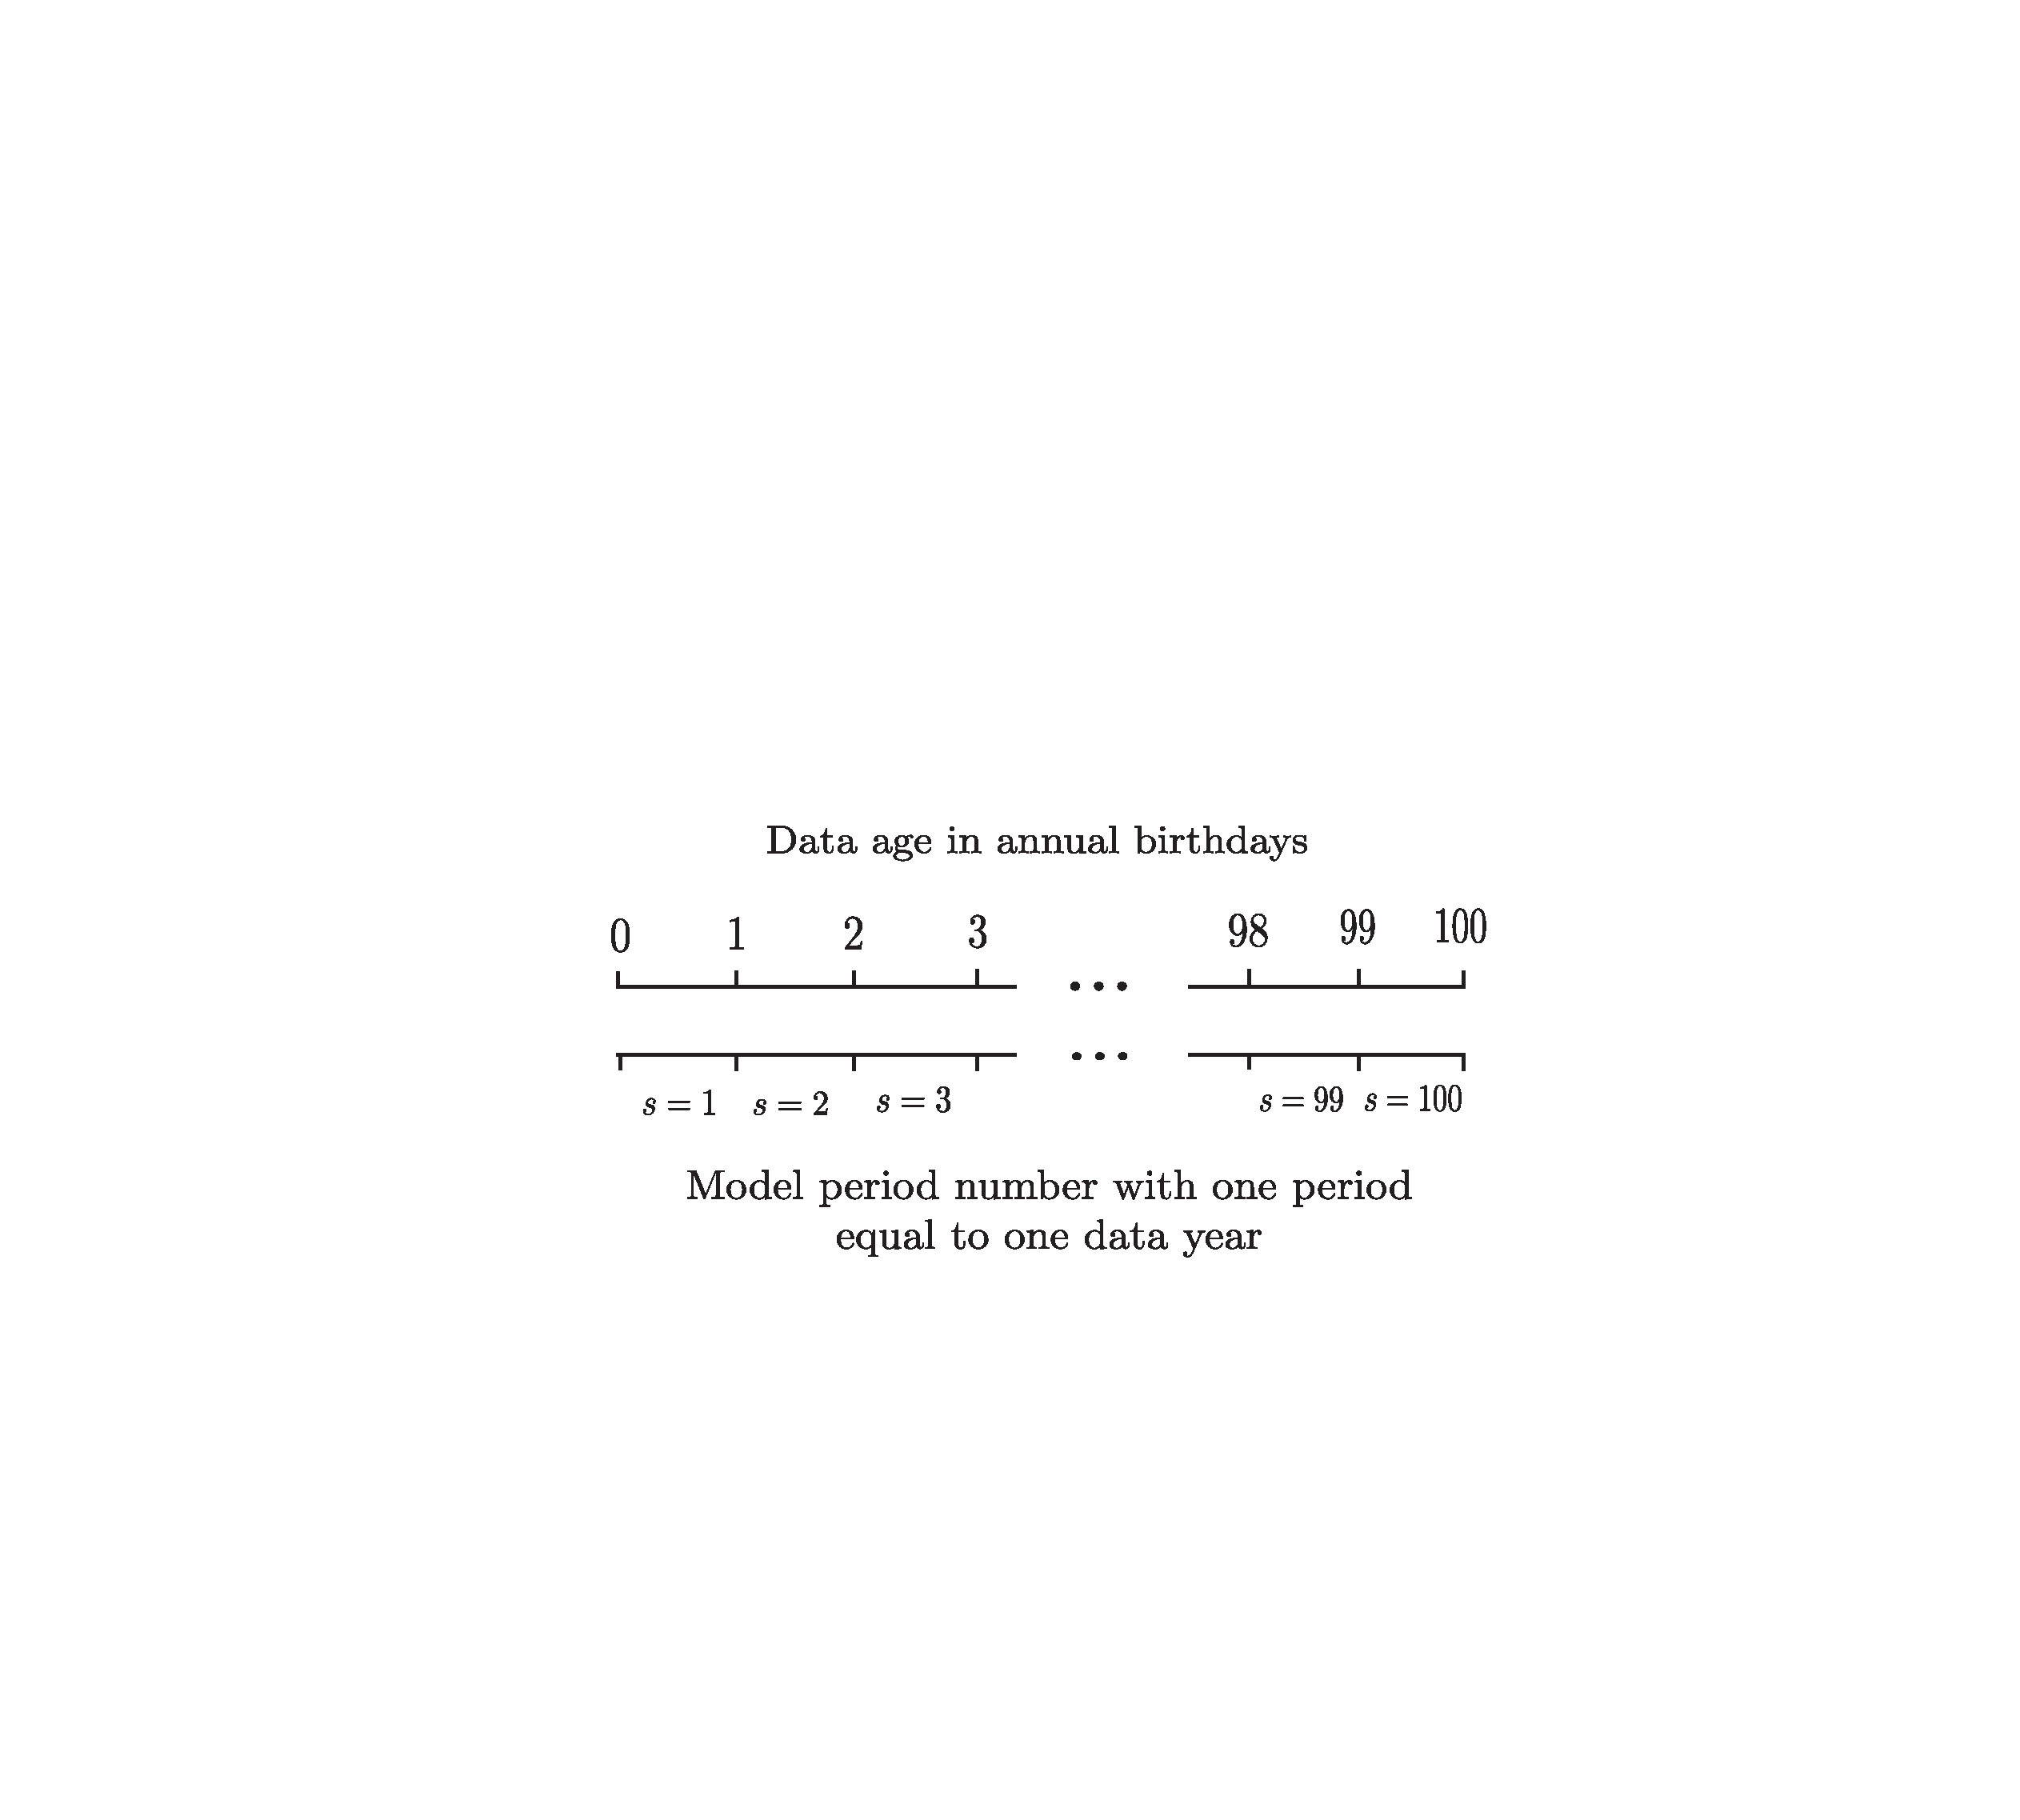
\includegraphics{images/FigPerTime.pdf}}}
  \end{figure}

  Our initial population distribution $\{\omega_{s,1}\}_{s=1}^{100}$ in Figure \ref{FigInitPopDist} comes from \citet{Census:2014} population estimates for both sexes for 2013. The fertility rates $\{f_s\}_{s=1}^{100}$ in Figure \ref{FigFertRates} come from \citet[Table 1]{NVSR:2010}. The mortality rates $\{\rho_s\}_{s=1}^{99}$ in Figure \ref{FigMortRates} come from the 2010 death probabilities in \citet{SocSec:2010}. We enforce a strict maximum age mortality rate of $\rho_{100}=1$ in our model.

  \begin{figure}[htbp]\centering \captionsetup{width=4.0in}
    \caption{\label{FigInitPopDist}\textbf{Initial population distribution $\omega_{s,1}$ by year, $1\leq s\leq 100$}}
    \fbox{\resizebox{4.0in}{2.8in}{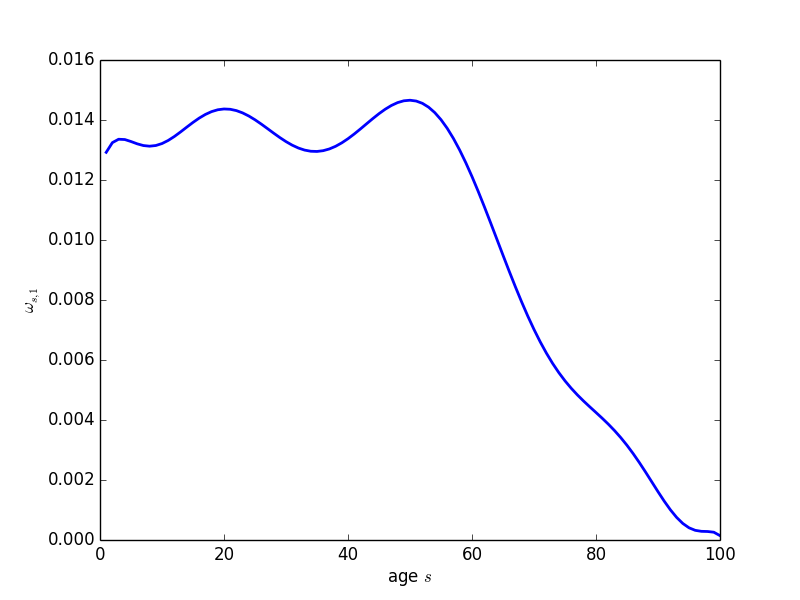
\includegraphics{images/omega_init.png}}}
  \end{figure}

  \begin{figure}[htbp]\centering \captionsetup{width=4.0in}
    \caption{\label{FigFertRates}\textbf{Fertility rates $f_s$ by year, $1\leq s\leq 100$}}
    \fbox{\resizebox{4.0in}{2.8in}{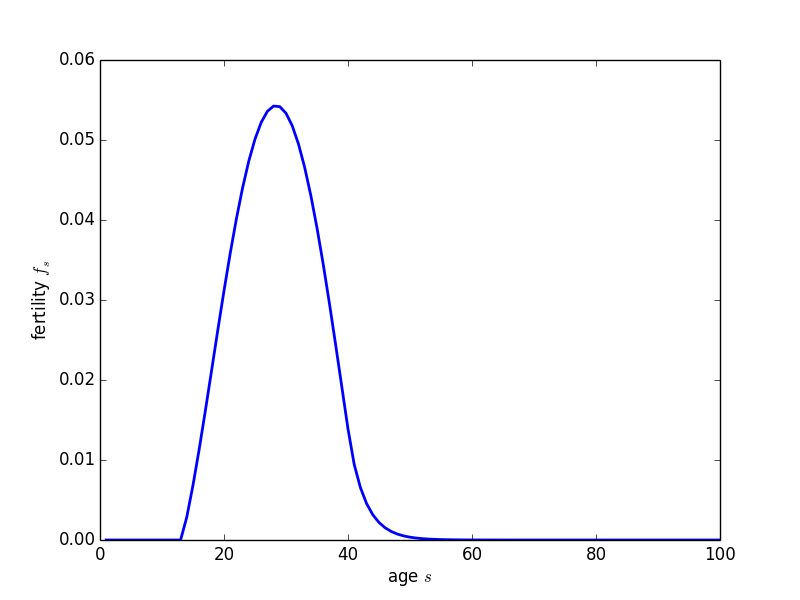
\includegraphics{images/fert_rates.png}}}
  \end{figure}

  \begin{figure}[htbp]\centering \captionsetup{width=4.0in}
    \caption{\label{FigMortRates}\textbf{Mortality rates $\rho_s$ by year, $1\leq s\leq 100$}}
    \fbox{\resizebox{4.0in}{2.8in}{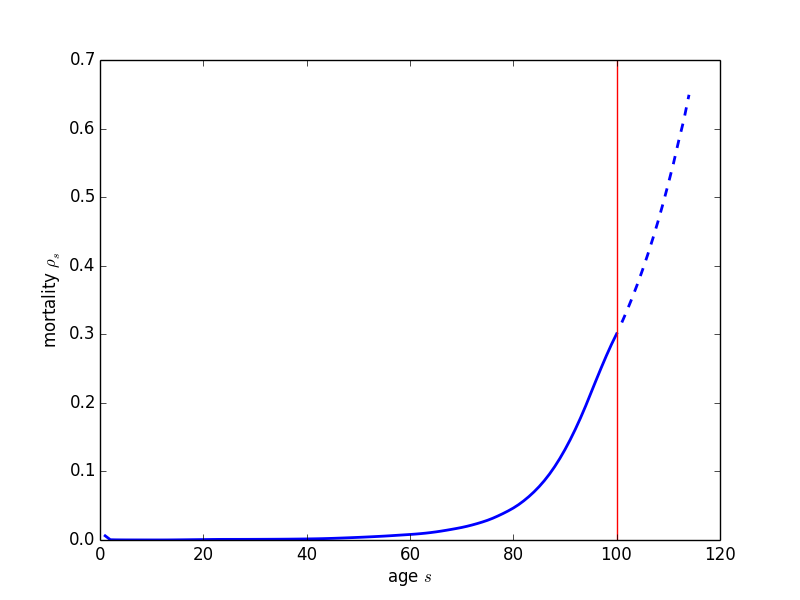
\includegraphics{images/mort_rates.png}}}
  \end{figure}

  The immigration rates $\{i_s\}_{s=1}^{99}$ in Figure \ref{FigImmigRates} are essentially residuals. We take total population for two consecutive years $N_t$ and $N_{t+1}$ and the population distribution by age in both of those years $\bm{\omega}_{t}$ and $\bm{\omega}_{t+1}$from the \citet{Census:2014} data. We then deduce the immigration rates $\{i_s\}_{s=1}^{99}$ using equation \eqref{EqPopLawofmotionStat}. We do this for three consecutive sets of years, so that our calibrated immigration rates by age are the average of our three years of deduced rates from the data for each age.

  \begin{figure}[htbp]\centering \captionsetup{width=4.0in}
    \caption{\label{FigImmigRates}\textbf{Immigration rates $i_s$ by year, $1\leq s\leq 100$}}
    \fbox{\resizebox{4.0in}{2.8in}{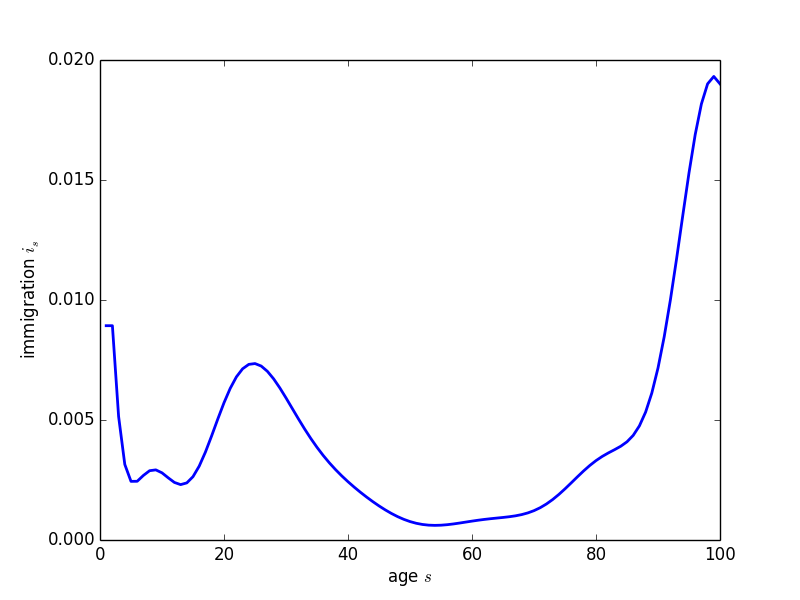
\includegraphics{images/imm_rates.png}}}
  \end{figure}

  Figure \ref{FigPopPath} shows the predicted time path of the total population $N_t$ given $\omega_{s,1}$ $f_s$, $i_s$, and $\rho_s$. Notice that the population approaches a constant growth rate. This is a result of the stationary population percent distribution $\bm{\bar{\omega}}$ eventually being reached. Figure \ref{FigSSpopdist} shows the steady-state population percent distribution by age $\bm{\bar{\omega}}$.

  \begin{figure}[htbp]\centering \captionsetup{width=4.0in}
    \caption{\label{FigPopPath}\textbf{Forecast time path of population growth rate $g_{n,t}$}}
    \fbox{\resizebox{4.0in}{2.8in}{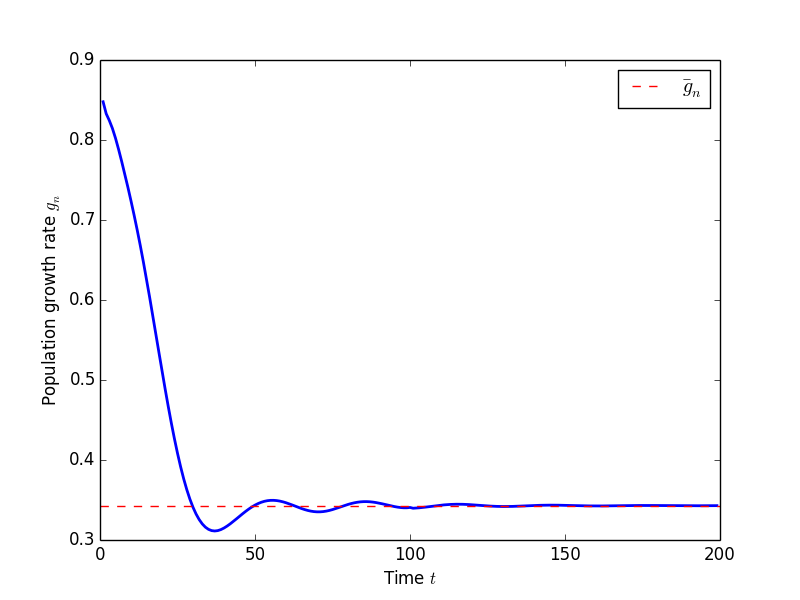
\includegraphics{images/Population_growthrate.png}}}
  \end{figure}

  \begin{figure}[htbp]\centering \captionsetup{width=4.0in}
    \caption{\label{FigSSpopdist}\textbf{Steady-state population percent distribution by age $\bm{\bar{\omega}}$}}
    \fbox{\resizebox{4.0in}{2.8in}{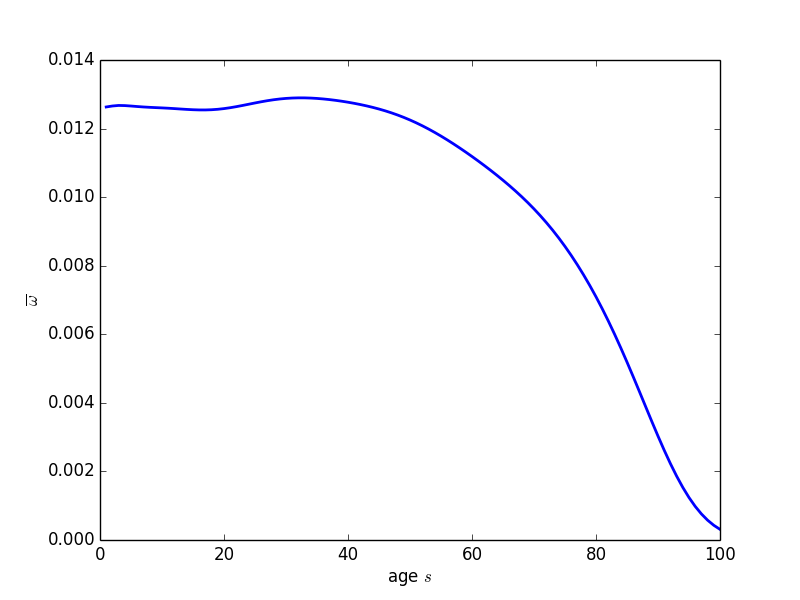
\includegraphics{images/omega_ss.png}}}
  \end{figure}
  \clearpage



\newpage
\section{Derivation of elliptical disutility of labor supply}\label{AppEllipseUtil}

  \setcounter{equation}{0}

  \citet{EvanPhillips:2015} provide an exposition of the value of using elliptical disutility of labor specification as well as its relative properties to such standard disutility of labor functions such as constant relative risk aversion (CRRA) and constant Frisch elasticity (CFE). A standard specification of additively separable period utility in consumption and labor supply first used in \citet{KPR:1988} is the following,
  \begin{equation}\label{AppEqStandUtil}
    u(c,n) = \frac{c^{1-\sigma} - 1}{1-\sigma} + \chi^n\frac{\left(\tilde{l} - n\right)^{1+\theta}}{1+\theta}
  \end{equation}
  where $\sigma\geq 1$ is the coefficient of relative risk aversion on consumption, $\theta\geq 0$ is proportional to the inverse of the Frisch elasticity of labor supply, and $\tilde{l}$ is the time endowment or the maximum labor supply possible. The constant $\chi^n$ is a scale parameter influencing the relative disutility of labor to the utility of consumption.

  Although labor supply is only defined for $n\in[0,\tilde{l}]$, the marginal utility of leisure at $n=\tilde{l}$ is infinity and is not defined for $n>\tilde{l}$. However, utility of labor in this functional form is defined for $n<0$. To avoid the well known and significant computational difficulty of computing the solution to the complementary slackness conditions in the Karush, Kuhn, Tucker constrained optimization problem, we impose an approximating utility function that has properties bounding the solution for $n$ away from both $n=\tilde{l}$ and $n=0$. The upper right quadrant of an ellipse has exactly this property and also has many of the properties of the original utility function. Figure \ref{FigUtilCompar} shows how our estimated elliptical utility function compares to the utility of labor from \eqref{AppEqStandUtil} over the allowed support of $n$.

  \begin{figure}[htb]\centering \captionsetup{width=4.0in}
    \caption{\label{FigUtilCompar}\textbf{Comparison of standard utility of labor $n$ to elliptical utility}}
    \fbox{\resizebox{4.0in}{3.2in}{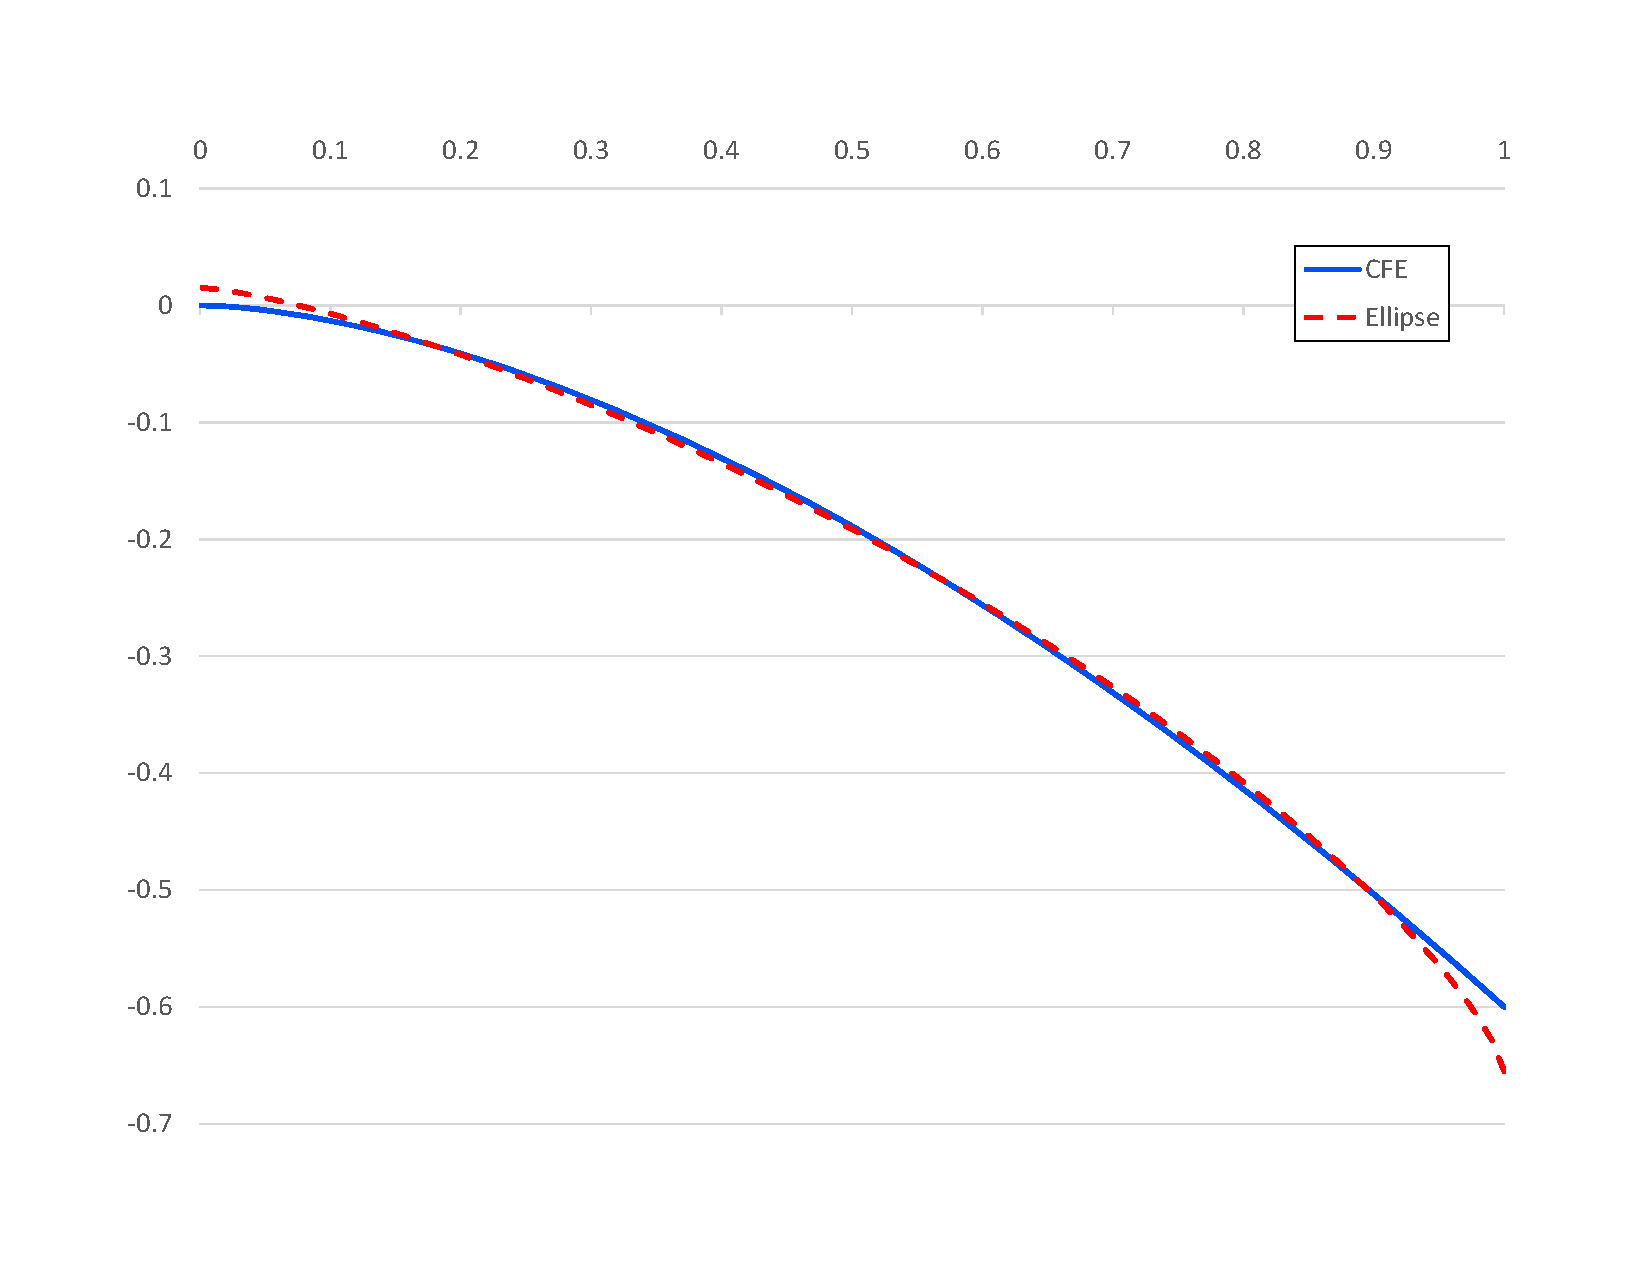
\includegraphics{images/EllipseUtilComp.pdf}}}
  \end{figure}

  The general equation for an ellipse in $x$ and $y$ space with centroid at coordinates $(h,k)$, horizontal radius of $a$, vertical radius of $b$, and curvature $\upsilon$ is the following.
  \begin{equation}\label{AppEqEllipseGen}
    \left(\frac{x - h}{a}\right)^\upsilon + \left(\frac{y - k}{b}\right)^\upsilon = 1
  \end{equation}
  Figure \ref{FigEllipseGen} shows an ellipse with the parameterization $[h,k,a,b,\upsilon]=[1,-1,1,2,2]$.

  \begin{figure}[htb]\centering \captionsetup{width=3.0in}
    \caption{\label{FigEllipseGen}\textbf{Ellipse with $[h,k,a,b,\upsilon]=[1,-1,1,2,2]$}}
    \fbox{\resizebox{3.0in}{3.8in}{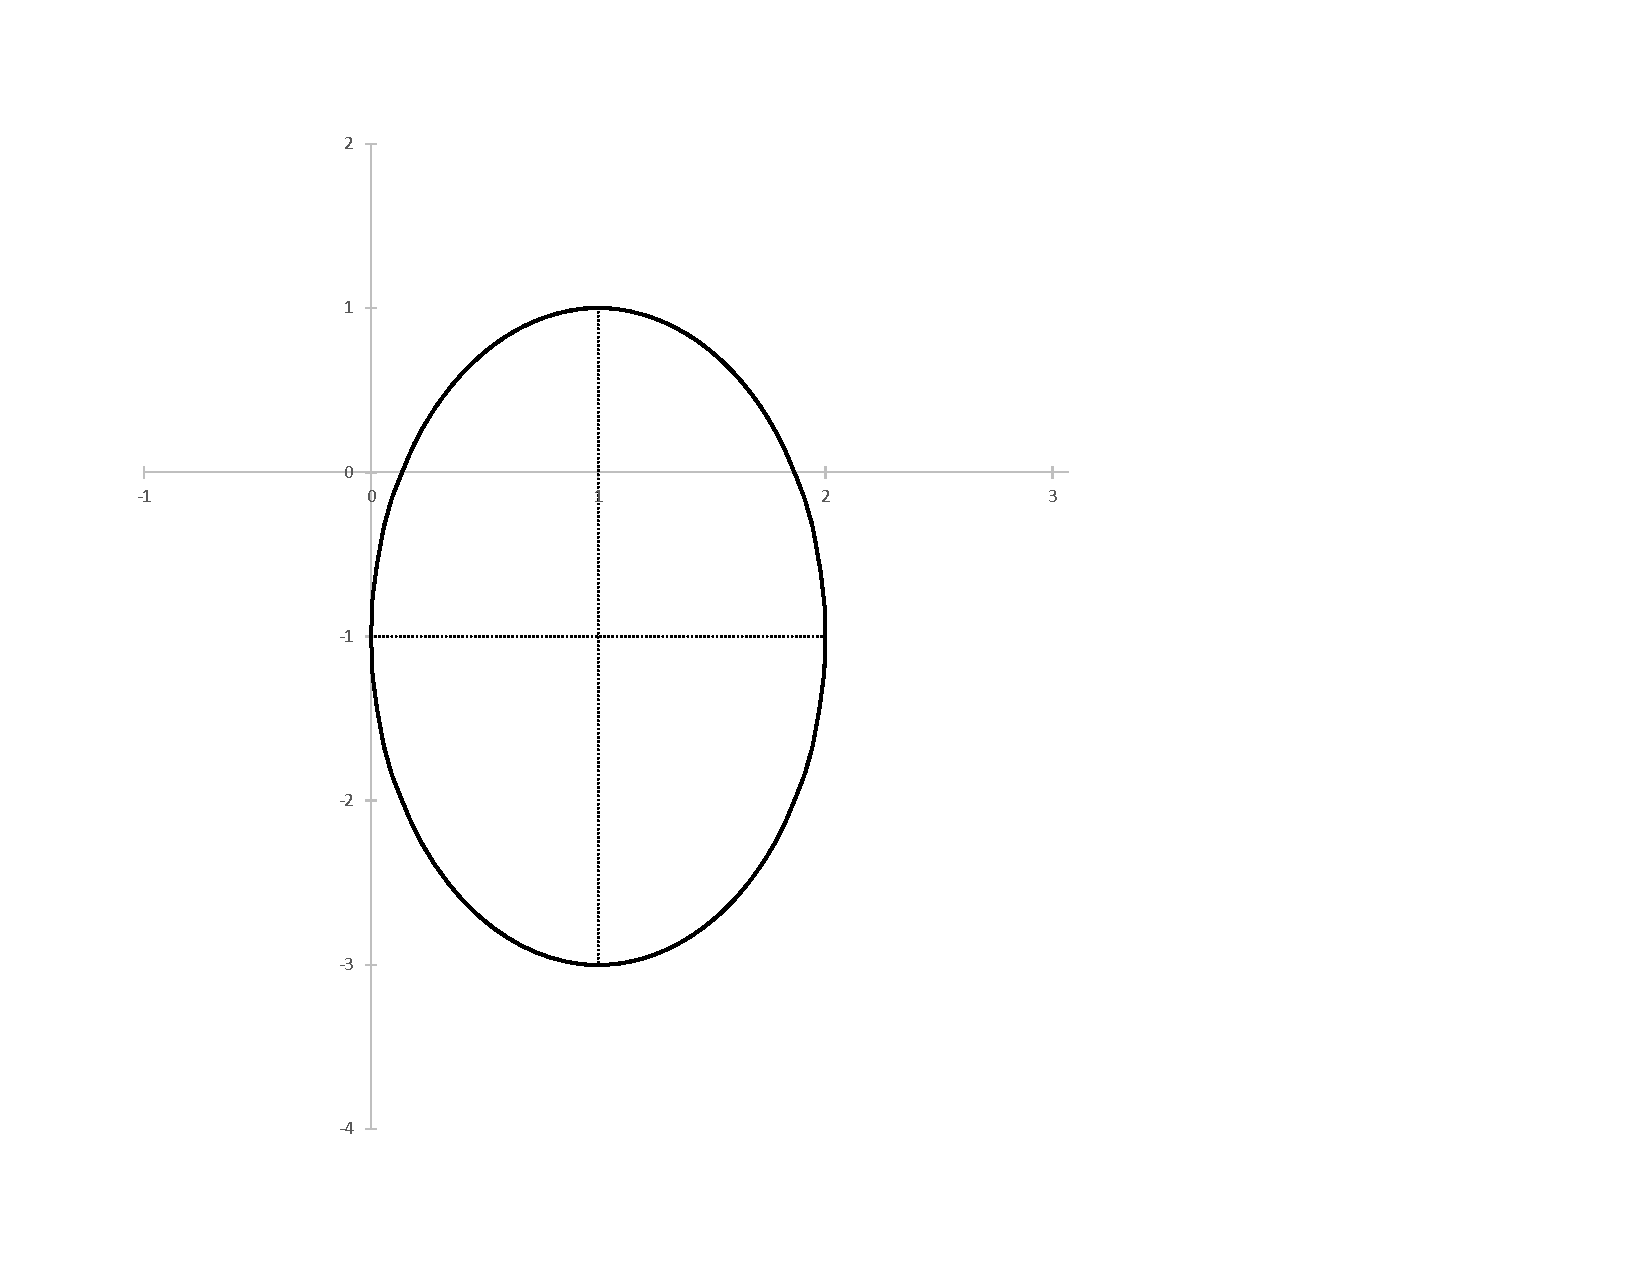
\includegraphics{images/EllipseGen2.pdf}}}
  \end{figure}

  The graph of the ellipse in the upper-right quadrant of Figure \ref{FigEllipseGen} ($x\in[1,2]$ and $y\in[-1,1]$) has similar properties to the utility of labor term in \eqref{AppEqStandUtil}. If we let the $x$ variable be labor supply $n$, the utility of labor supply be $g(n)$, the $x$-coordinate of the centroid be zero $h=0$, and the horizontal radius of the ellipse be $a=\tilde{l}$, then the equation for the ellipse corresponding to the standard utility specification is the following.
  \begin{equation}\label{AppEqEllipseN}
    \left(\frac{n}{\tilde{l}}\right)^\upsilon + \left(\frac{g - k}{b}\right)^\upsilon = 1
  \end{equation}
  Solving the equation for $g$ as a function of $n$, we get the following.
  \begin{equation}\label{AppEqGn}
    g(n) = b\left[1 - \left(\frac{n}{\tilde{l}}\right)^\upsilon\right]^{\frac{1}{\upsilon}} + k
  \end{equation}
  The $\upsilon$ parameter acts like a constant elasticity of substitution, and the parameter $b$ is a shape parameter similar to $\chi^n$ in \eqref{AppEqStandUtil}.

  We use the upper-right quadrant of the elliptical utility function because the utility of $n$ is strictly decreasing on $n\in(0,\tilde{l})$, because the slope of the utility function goes to negative infinity as $n$ approaches its maximum of $\tilde{l}$ and because the slope of the utility function goes to zero as $n$ approaches its minimum of 0. This creates interior solutions for all optimal labor supply choices $n^*\in(0,\tilde{l})$. Although it is more realistic to allow optimal labor supply to sometimes be zero, the complexity and dimensionality of our model requires this approximating assumption to render the solution method tractable.

  Figure \ref{FigUtilCompar} shows how closely the estimated elliptical utility function matches the original utility of labor function in \eqref{AppEqStandUtil} with a Frish elasticity of 1.5\footnote{See \citet{Chetty:2011}, \citet{KeaneRogerson:2012} and \citet{Peterman:2014} for discussion of this choice.} . We choose the ellipse parameters $b$, $k$, and $\upsilon$ to best match the points on the original utility of labor function for $n\in[0,1]$. We minimize the sum of absolute errors for 101 evenly spaced points on this domain. The estimated values of the parameters for the elliptical utility shown in Figure \ref{FigUtilCompar} and represented in equation \eqref{AppEqGn} are $[b,k,\upsilon] = [.6701,-.6548,1.3499]$.

  \clearpage


\newpage
\section{Solving for stationary steady-state equilibrium}\label{AppSSsolve}

  \setcounter{equation}{0}
  \renewcommand\theenumi{\arabic{enumi}}
  \renewcommand\theenumii{\alph{enumii}}
  \renewcommand\theenumiii{\roman{enumiii}}

  This section describes the solution method for the stationary steady-state equilibrium described in Definition \ref{DefEquilSS}.

  \begin{enumerate}
    \item Use the techniques in Appendix \ref{AppPopGrowth} to solve for the steady-state population distribution vector $\bm{\bar{\omega}}$ of the exogenous population process.
    \item Choose an initial guess for the stationary steady-state distribution of capital $\bar{b}_{j,s+1}$ for all $j$ and $s=E+2,E+3,...E+S+1$ and labor supply $\bar{n}_{j,s}$ for all $j$ and $s$.
      \begin{itemize}
        \item A good first guess is a large positive number for all the $\bar{n}_{j,s}$ that is slightly less than $\tilde{l}$ and to choose some small positive number for $\bar{b}_{j,s+1}$ that is small enough to be less than the minimum income that an individual might have $\bar{w}e_{j,s}\bar{n}_{j,s}$.
      \end{itemize}
    \item Perform an unconstrained root finder that chooses $\bar{n}_{j,s}$ and $\bar{b}_{j,s+1}$ that solves the $2JS$ stationary steady-state Euler equations.
    \item Make sure none of the implied steady-state consumptions $\bar{c}_{j,s}$ is less-than-or-equal-to zero.
      \begin{itemize}
        \item If one consumption is less-than-or-equal-to zero $\bar{c}_{j,s}\leq 0$, then try different starting values.
      \end{itemize}
    \item Make sure that none of the Euler errors is too large in absolute value for interior stationary steady-state values. A steady-state Euler error is the following, which is supposed to be close to zero for all $j$ and $s$:
      \begin{align}
        \begin{split}
          &\frac{\chi^n_{s}\left(\frac{b}{\tilde{l}}\right)\left(\frac{\bar{n}_{j,s}}{\tilde{l}}\right)^{\upsilon-1}\left[1 - \left(\frac{\bar{n}_{j,s}}{\tilde{l}}\right)^\upsilon\right]^{\frac{1-\upsilon}{\upsilon}}}{(\bar{c}_{j,s})^{-\sigma}\left(\bar{w} e_{j,s} - \frac{\partial\bar{T}_{j,s}}{\partial \bar{n}_{j,s}}\right)} - 1 \\
          &\qquad\qquad\qquad\qquad\qquad\qquad\qquad\forall j\quad\text{and}\quad E+1\leq s\leq E+S
        \end{split} \label{EqSSeulerrLab} \\
        \begin{split}
          &\frac{e^{-g_y\sigma}\left(\rho_s\chi^b_j \left(\bar{b}_{j,s+1}\right)^{-\sigma} + \beta(1-\rho_s)(\bar{c}_{j,s+1})^{-\sigma}\left[(1 + \bar{r}) - \frac{\partial \bar{T}_{j,s+1}}{\partial \bar{b}_{j,s+1}}\right]\right)}{(\bar{c}_{j,s})^{-\sigma}} - 1 \\
          &\qquad\qquad\qquad\qquad\qquad\qquad\qquad\forall j \quad\text{and}\quad E+1\leq s\leq E+S-1 \\
        \end{split} \label{EqSSeulerrSav} \\
        &\frac{\chi^b_j e^{-g_y\sigma}(\bar{b}_{j,E+S+1})^{-\sigma}}{\left(\bar{c}_{j,E+S}\right)^{-\sigma}} - 1 \quad\forall j \label{EqSSeulerrBeq}
      \end{align}
  \end{enumerate}


\newpage
\section{Solving for stationary non-steady-state equilibrium by time path iteration}\label{AppNonSSsolve}

  \setcounter{equation}{0}

  This section defines the non-steady-state transition path equilibrium of the model and outlines the benchmark time path iteration (TPI) method of \citet{AuerbachKotlikoff:1987} for solving the stationary non-steady-state equilibrium transition path of the distribution of savings. The definition of the stationary non-steady-state equilibrium is similar to Definition \ref{DefEquilSS}, with the stationary steady-state equilibrium definition being a special case of the stationary non-steady-state equilibrium.

  \vspace{7mm}

  \hrule
  \begin{definition}[\textbf{Stationary non-steady-state equilibrium}]\label{DefEquilNonSS}
    A non-autarkic stationary non-steady-state equilibrium in the overlapping generations model with $S$-period lived agents and heterogeneous ability $e_{j,s}$ is defined as allocations $n_{j,s,t}$ and $\hat{b}_{j,s+1,t+1}$ and prices $\hat{w}_t$ and $r_t$ for all $j$, $s$, and $t$ such that the following conditions hold:
     \begin{enumerate}
        \item individuals have symmetric beliefs $\Omega(\cdot)$ about the evolution of the distribution of savings, and those beliefs about the future distribution of savings equal the realized outcome (rational expectations),
          \begin{equation*}
            \bm{\hat{\Gamma}}_{t+u} = \bm{\hat{\Gamma}}^e_{t+u} = \Omega^u\left( \bm{\hat{\Gamma}}_t\right) \quad\forall t, \quad u\geq 1
          \end{equation*}
        \item individuals optimize according to \eqref{EqEulerLabStat}, \eqref{EqEulerSavStat}, and \eqref{EqEulerSavEpSstat}
        \item Firms optimize according to \eqref{EqFOCwageStat} and \eqref{EqFOCrate}, and
        \item Markets clear according to \eqref{EqMktClrLabStat} and \eqref{EqMktClrCapStat}.
     \end{enumerate}
  \end{definition}
  \hrule

  \vspace{10mm}

  \noindent Taken together, the individual labor-leisure and intended bequest decisions in the last period of life show that the optimal labor supply and optimal intended bequests for age $s=E+S$ are each functions of individual savings, total bequests received, and the prices in that period: $n_{j,E+S,t}=\phi\bigl(\hat{b}_{j,E+S,t},\hat{BQ}_{j,t},\hat{w}_t,r_t\bigr)$ and $\hat{b}_{j,E+S+1,t+1}=\psi\bigl(\hat{b}_{j,E+S,t},\hat{BQ}_{j,t},\hat{w}_t,r_t\bigr)$. These two decisions are characterized by final-age version of the static labor supply Euler equation \eqref{EqEulerLabStat} and the static intended bequests Euler equation \eqref{EqEulerSavEpSstat}. individuals in their second-to-last period of life in period $t$ have four decisions to make. They must choose how much to work this period, $n_{j,E+S-1,t}$, and next period, $n_{j,E+S,t+1}$, how much to save this period for next period, $\hat{b}_{j,E+S,t+1}$, and how much to bequeath next period, $\hat{b}_{j,E+S+1,t+2}$. The optimal responses for this individual are characterized by the $s=E+S-1$ and $s=E+S$ versions of the static Euler equations \eqref{EqEulerLabStat}, the $s=E+S-1$ version of the intertemporal Euler equation \eqref{EqEulerSavStat}, and the $s=E+S$ static bequest Euler equation \eqref{EqEulerSavEpSstat}, respectively.

  Optimal savings in the second-to-last period of life $s=E+S-1$ is a function of the current savings as well as the total bequests received and prices in the current period and in the next period $\hat{b}_{j,E+S,t+1} = \psi\bigl(\hat{b}_{j,E+S-1,t},\hat{BQ}_{j,t},\hat{w}_t,r_t,\hat{BQ}_{j,t+1},\hat{w}_{t+1},r_{t+1}|\Omega\bigr)$ given beliefs $\Omega$. As before, the optimal labor supply at age $s=E+S$ is a function of the next period's savings, bequests received, and prices.
  \begin{equation*}
    n_{j,E+S,t+1}=\phi\bigl(\hat{b}_{j,E+S,t+1},\hat{BQ}_{j,t+1},\hat{w}_{t+1},r_{t+1}\bigr)
  \end{equation*}
  But the optimal labor supply at age $s=E+S-1$ is a function of the current savings, current bequests received, and the current prices as well as the future bequests received and future prices because of the dependence on the savings decision in that same period $n_{j,E+S-1,t}=\phi\bigl(\hat{b}_{j,E+S-1,t},\hat{BQ}_{j,t},\hat{w}_t,r_t,\hat{BQ}_{j,t+1},\hat{w}_{t+1},r_{t+1}|\Omega\bigr)$ given beliefs $\Omega$. By induction, we can show that the optimal labor supply, savings, and intended bequests functions for any individual with ability $j$, age $s$, and in period $t$ is a function of current holdings of savings and the lifetime path of total bequests received and prices given beliefs $\Omega$.
  \begin{align}
    n_{j,s,t} &= \phi\Bigl(\hat{b}_{j,s,t},\bigl(\hat{BQ}_{j,v},\hat{w}_v,r_v\bigr)_{v=t}^{t+S-s}|\Omega\Bigr) \quad\forall j,s,t \label{EqLabPolFuncGen} \\
    \hat{b}_{j,s+1,t+1} &= \psi\Bigl(\hat{b}_{j,s,t},\bigl(\hat{BQ}_{j,v},\hat{w}_v,r_v\bigr)_{v=t}^{t+S-s}|\Omega\Bigr) \quad\forall j,t \quad\text{and}\quad E+1\leq s\leq E+S \label{EqSavPolFuncGen}
  \end{align}

  If one knows the current distribution of individuals savings and intended bequests, $\bm{\hat{\Gamma}}_t$, and beliefs about $\bm{\hat{\Gamma}}_t$, then one can predict time series for total bequests received $\hat{BQ}_{j,t}$, real wages $\hat{w}_t$ and real interest rates $r_t$ necessary for solving each individual's optimal decisions. Characteristic (i) in equilibrium definition \ref{DefEquilNonSS} implies that individuals be able to forecast prices with perfect foresight over their lifetimes implies that each individual has correct information and beliefs about all the other individuals optimization problems and information. It also implies that the equilibrium allocations and prices are really just functions of the entire distribution of savings at a particular period, as well as a law of motion for that distribution of savings.

  In equilibrium, the steady-state individual labor supply, $\bar{n}_{j,s}$, for all $j$ and $s$, the steady-state savings, $\bar{b}_{j,E+S+1}$, the steady-state real wage, $\bar{w}$, and the steady-state real rental rate, $\bar{r}$, are simply functions of the steady-state distribution of savings $\bar{\Gamma}$. This is clear from the steady-state version of the capital market clearing condition \eqref{EqMktClrCapStat} and the fact that aggregate labor supply is a function of the sum of exogenous efficiency units of labor in the labor market clearing condition \eqref{EqMktClrLabStat}. The two firm first order conditions for the real wage $\hat{w}_t$ \eqref{EqFOCwageStat} and real rental rate $r_t$ \eqref{EqFOCrate} are only functions of the stationary aggregate capital stock $\hat{K}_t$ and aggregate labor $\hat{L}_t$.

  \begin{figure}[htb]\centering \captionsetup{width=4.0in}
    \caption{\label{FigKpathTPI}\textbf{Equilibrium time path of $K_t$ for $S=80$ and $J=7$ in baseline model}}
    \fbox{\resizebox{4.0in}{3.0in}{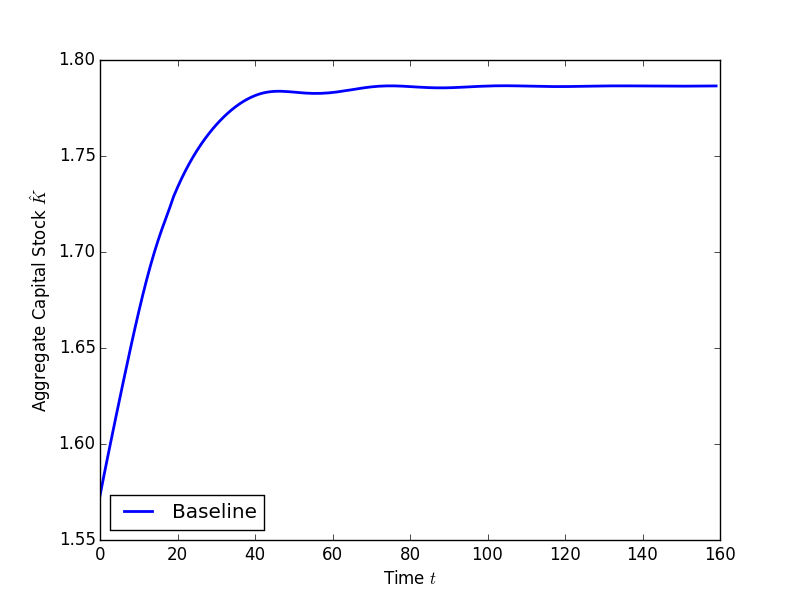
\includegraphics{images/TPI_K.png}}}
  \end{figure}

  \begin{figure}[htb]\centering \captionsetup{width=4.0in}
    \caption{\label{FigLpathTPI}\textbf{Equilibrium time path of $L_t$ for $S=80$ and $J=7$ in baseline model}}
    \fbox{\resizebox{4.0in}{3.0in}{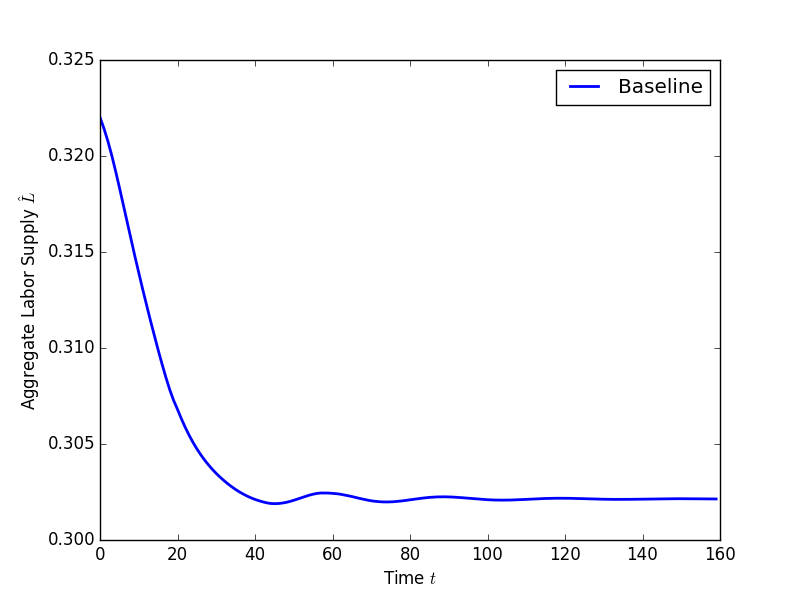
\includegraphics{images/TPI_L.png}}}
  \end{figure}

  To solve for any stationary non-steady-state equilibrium time path of the economy from an arbitrary current state to the steady state, we follow the time path iteration (TPI) method of \citet{AuerbachKotlikoff:1987}. The approach is to choose an arbitrary time path for the stationary aggregate capital stock $\hat{K}_t$, stationary aggregate labor $\hat{L}_t$, and total bequests received $\hat{BQ}_{j,t}$ for each type $j$. This initial guess of a path implies arbitrary beliefs that violate the rational expectations requirement. We then solve for individuals' optimal decisions given the time paths of those variables, which decisions imply new time paths of those variables. We then update the time path as a convex combination of the initial guess and the new implied path. Figures \ref{FigKpathTPI} and \ref{FigLpathTPI} show the equilibrium time paths of the aggregate capital stock and aggregate labor, respectively, for the calibration described in Table \ref{TabExogVars} for $T=160$ periods starting from an initial distribution of savings in which $b_{j,s,1}=\bm{\bar{\Gamma}}$ for all $j$ and $s$ in the case that no policy experiment takes place. The initial capital stock $\hat{K}_1$ is not at the steady state $\bar{K}$ because the initial population distribution is not at the steady-state.

  The computational approach to solving for the non-steady-state transition path equilibrium is the time path iteration (TPI) method of \citet{AuerbachKotlikoff:1987}. TPI finds a fixed point for the transition path of the distribution of capital for a given initial state of the distribution of capital. The idea is that the economy is infinitely lived, even though the agents that make up the economy are not. Rather than recursively solving for equilibrium policy functions by iterating on individual value functions, one must recursively solve for the policy functions by iterating on the entire transition path of the endogenous objects in the economy (see \citet[ch. 17]{StokeyLucas:1989}).

  The key assumption is that the economy will reach the steady-state equilibrium described in Definition \ref{DefEquilSS} in a finite number of periods $T<\infty$ regardless of the initial state. Let $\bm{\hat{\Gamma}}_t$ represent the distribution of stationary savings at time $t$.
  \begin{equation}\tag{\ref{EqSavDist}}
    \bm{\hat{\Gamma}}_t \equiv \Bigl\{\bigl\{\hat{b}_{j,s,t}\bigr\}_{j=1}^J\Bigr\}_{s=E+2}^{E+S+1}, \quad\forall t
  \end{equation}
  In Section \ref{SecMCEqlbm}, we describe how the stationary non-steady-state equilibrium time path of allocations and price is characterized by functions of the state $\bm{\hat{\Gamma}}_t$ and its law of motion. TPI starts the economy at any initial distribution of savings $\bm{\hat{\Gamma}}_1$ and solves for its equilibrium time path over $T$ periods to the steady-state distribution $\bm{\bar{\Gamma}}_T$.

  The first step is to assume an initial transition path for aggregate stationary capital $\bm{\hat{K}}^i = \left\{\hat{K}_1^i,\hat{K}_2^i,...\hat{K}_T^i\right\}$, aggregate stationary labor $\bm{\hat{L}}^i = \left\{\hat{L}_1^i,\hat{L}_2^i,...\hat{L}_T^i\right\}$, and total bequests received $\bm{\hat{BQ}}_j^i=\{\hat{BQ}_{j,1}^i,\hat{BQ}_{j,2}^i,...\hat{BQ}_{j,T}^i\}$ for each ability type $j$ such that $T$ is sufficiently large to ensure that $\bm{\hat{\Gamma}}_T = \bar{\bm{\Gamma}}$, $\hat{K}_T^i\left(\bm{\Gamma}_T\right)$, $\hat{L}_T^i\left(\bm{\Gamma}_T\right) = \bar{L}\left(\bar{\bm{\Gamma}}\right)$, and $\hat{BQ}_{j,T}^i\left(\bm{\Gamma}_T\right) = \bar{BQ}_j\left(\bar{\bm{\Gamma}}\right)$ for all $t\geq T$. The superscript $i$ is an index for the iteration number. The transition paths for aggregate capital and aggregate labor determine the transition paths for both the real wage $\bm{\hat{w}}^i = \left\{\hat{w}_1^i,\hat{w}_2^i,...\hat{w}_T^i\right\}$ and the real return on investment $\bm{r}^i = \left\{r_1^i,r_2^i,...r_T^i\right\}$. The time paths for the total bequests received also figure in each period's budget constraint and are determined by the distribution of savings and intended bequests.

  The exact initial distribution of capital in the first period $\bm{\hat{\Gamma}}_1$ can be arbitrarily chosen as long as it satisfies the stationary capital market clearing condition \eqref{EqMktClrCapStat}.
  \begin{equation}\label{EqMktClrCapStat1}
    \hat{K}_1 = \frac{1}{1 + \tilde{g}_{n,1}}\sum_{s=E+2}^{E+S+1}\sum_{j=1}^{J}\hat{\omega}_{s-1,0}\lambda_j \hat{b}_{j,s,1}
  \end{equation}
  Simiilarly, each initial value of total bequests received $\hat{BQ}_{j,1}^i$ must be consistent with the initial distribution of capital through the stationary version of \eqref{EqTotBeq}.
  \begin{equation}\label{EqTotBeqStat1}
    \hat{BQ}_{j,1} = \frac{(1+r_1)\lambda_j}{1+\tilde{g}_{n,1}}\sum_{s=E+1}^{E+S}\rho_s\hat{\omega}_{s,0}\hat{b}_{j,s+1,1} \quad\forall j
  \end{equation}
  However, this is not the case with $\hat{L}_1^i$. Its value will be endogenously determined in the same way the $K_2^i$ is. For this reason, a logical initial guess for the time path of aggregate labor is the steady state in every period $L_t^1 = \bar{L}$ for all $1\leq t\leq T$.

  It is easiest to first choose the initial distribution of savings $\bm{\hat{\Gamma}}_1$ and then choose an initial aggregate capital stock $\hat{K}_1^i$ and initial total bequests received $\hat{BQ}_{j,1}^i$ that correspond to that distribution. As mentioned earlier, the only other restrictions on the initial transition paths for aggregate capital, aggregate labor, and total bequests received is that they equal their steady-state levels $\hat{K}_T^i = \bar{K}\left(\bm{\bar{\Gamma}}\right)$, $\hat{L}_T^i = \bar{L}\left(\bm{\bar{\Gamma}}\right)$, and $\hat{BQ}_{j,T}^i = \bar{BQ}_j\left(\bm{\bar{\Gamma}}\right)$ by period $T$. \citet{EvansPhillips:2014} have shown that the initial guess for the aggregate capital stocks $\hat{K}_t^i$ for periods $1<t<T$ can take on almost any positive values satisfying the constraints above and still have the time path iteration converge.

  Given the initial savings distribution $\bm{\hat{\Gamma}}_1$ and the transition paths of aggregate capital $\bm{\hat{K}}^i = \left\{\hat{K}_1^i,\hat{K}_2^i,...\hat{K}_T^i\right\}$, aggregate labor $\bm{\hat{L}}^i = \left\{\hat{L}_1^i,\hat{L}_2^i,...\hat{L}_T^i\right\}$, and total bequests received $\bm{\hat{BQ}}_j^i = \left\{\hat{BQ}_{j,1}^i,\hat{BQ}_{j,2}^i,...\hat{BQ}_{j,T}^i\right\}$, as well as the resulting real wage $\bm{\hat{w}}^i = \left\{\hat{w}_1^i,\hat{w}_2^i,...\hat{w}_T^i\right\}$, and real return to savings $\bm{r}^i = \left\{r_1^i,r_2^i,...r_T^i\right\}$, one can solve for the period-1 optimal labor supply and intended bequests for each type $j$ of $s=E+S$-aged agents in the last period of their lives $n_{j,E+S,1}=\phi_{j,E+S}(\hat{b}_{j,E+S,1},\hat{BQ}_{j,E+S,1},\hat{w}_1,r_1)$ and $\hat{b}_{j,E+S+1,2}=\psi_{j,E+S}(\hat{b}_{j,E+S,1},\hat{BQ}_{j,E+S,1},\hat{w}_1,r_1)$ using his two $s=E+S$ static Euler equations \eqref{EqEulerLabStat} and \eqref{EqEulerSavEpSstat}.
  \begin{equation}\label{EqEulerSlabt1}
    \begin{split}
      &(\hat{c}_{j,E+S,1})^{-\sigma}\Biggl(\hat{w}_1^i e_{j,E+S} - \frac{\partial\hat{T}_{j,E+S,1}}{\partial n_{j,E+S,1}}\Biggr) = ... \\
      &\qquad\qquad\qquad\qquad \chi^n_{E+S}\biggl(\frac{b}{\tilde{l}}\biggr)\biggl(\frac{n_{j,E+S,1}}{\tilde{l}}\biggr)^{\upsilon-1}\Biggl[1 - \biggl(\frac{n_{j,E+S,1}}{\tilde{l}}\biggr)^\upsilon\Biggr]^{\frac{1-\upsilon}{\upsilon}} \quad\forall j \\
      &\quad\text{where}\quad \hat{c}_{j,E+S,1} = ... \\
      &\qquad\qquad\qquad \left(1 + r_1^i\right)\hat{b}_{j,E+S,1} + \hat{w}_1^i e_{j,E+S}n_{j,E+S,1} + \frac{\hat{BQ}_{j,1}}{\lambda_j} - e^{g_y}\hat{b}_{j,E+S+1,2} - \hat{T}_{j,E+S,1} \\
      &\quad\text{and}\quad \frac{\partial \hat{T}_{j,E+S,1}}{\partial n_{j,E+S,1}} = ... \\
      &\qquad\qquad\qquad \hat{w}_1^i e_{j,E+S}\biggl[\tau^I\bigl(F\hat{a}_{j,E+S,1}\bigr) + \frac{\hat{a}_{j,E+S,1}CDF\bigl[2A(F\hat{a}_{j,E+S,1})+B\bigr]}{\bigl[A(F\hat{a}_{j,E+S,1})^2+B(F \hat{a}_{j,E+S,1})+C\bigr]^2} + \tau^P\Biggr]
    \end{split}
  \end{equation}
  \begin{equation}\label{EqEulerSbeqt1}
    (\hat{c}_{j,E+S,1})^{-\sigma} = \chi^b_j e^{-g_y\sigma}(\hat{b}_{j,E+S+1,2})^{-\sigma} \quad\forall j
  \end{equation}
  Note that this is simply two equations \eqref{EqEulerSlabt1} and \eqref{EqEulerSbeqt1} and two unknowns $n_{j,E+S,1}$ and $\hat{b}_{j,E+S+1,2}$.

  We then solve the problem for all $j$ types of $E+S-1$-aged individuals in period $t=1$, each of which entails labor supply decisions in the current period $n_{j,E+S-1,1}$ and in the next period $n_{j,E+S,2}$, a savings decision in the current period for the next period $\hat{b}_{j,E+S,2}$ and an intended bequest decision in the last period $\hat{b}_{j,E+S+1,3}$. The labor supply decision in the initial period and the savings period in the initial period for the next period for each type $j$ of $E+S-1$-aged individuals are policy functions of the current savings and the total bequests received and prices in this period and the next $\hat{b}_{j,E+S,2} = \psi_{j,E+S-1}(\hat{b}_{j,E+S-1,1},\{\hat{BQ}_{j,t},\hat{w}_t,r_t\}_{t=1}^2)$ and $\hat{n}_{j,E+S-1,1} = \phi_{j,E+S-1}(\hat{b}_{j,E+S-1,1},\{\hat{BQ}_{j,t},\hat{w}_t,r_t\}_{t=1}^2)$. The labor supply and intended bequests decisions in the next period are simply functions of the savings, total bequests received, and prices in that period $\hat{n}_{j,E+S,2} = \phi_{j,E+S}(\hat{b}_{j,E+S,2},\hat{BQ}_{j,2},\hat{w}_2,r_2)$ and $\hat{b}_{j,E+S+1,3} = \psi_{j,E+S}(\hat{b}_{j,E+S,2},\hat{BQ}_{j,2},\hat{w}_2,r_2)$. These four functions are characterized by the following versions of equations \eqref{EqEulerLabStat}, \eqref{EqEulerSavStat}, and \eqref{EqEulerSavEpSstat}.
  \begin{equation}\label{EqEulerSm1labt1}
    \begin{split}
      &(\hat{c}_{j,E+S-1,1})^{-\sigma}\Biggl(\hat{w}_1^i e_{j,E+S-1} - \frac{\partial\hat{T}_{j,E+S-1,1}}{\partial n_{j,E+S-1,1}}\Biggr) = ... \\
      &\qquad\qquad\qquad \chi^n_{E+S-1}\biggl(\frac{b}{\tilde{l}}\biggr)\biggl(\frac{n_{j,E+S-1,1}}{\tilde{l}}\biggr)^{\upsilon-1}\Biggl[1 - \biggl(\frac{n_{j,E+S-1,1}}{\tilde{l}}\biggr)^\upsilon\Biggr]^{\frac{1-\upsilon}{\upsilon}} \quad\forall j
    \end{split}
  \end{equation}
  \begin{equation}\label{EqEulerSm1savt1}
    \begin{split}
      &(\hat{c}_{j,E+S-1,1})^{-\sigma} = ... \\
      &e^{-g_y\sigma}\Biggl(\rho_{E+S-1}\chi^b_j \bigl(\hat{b}_{j,E+S,2}\bigr)^{-\sigma} + \beta(1-\rho_{E+S-1})(\hat{c}_{j,E+S,2})^{-\sigma}\Biggl[(1 + r_2^i) - \frac{\partial T_{j,E+S,2}}{\partial b_{j,E+S,2}}\Biggr]\Biggr) \\
      &\qquad\qquad\qquad\qquad\qquad\qquad\qquad\qquad\qquad\qquad\qquad\qquad\qquad\qquad\qquad\qquad\forall j \\
      &\qquad\text{where}\quad \frac{\partial T_{j,E+S,2}}{\partial b_{j,E+S,2}} = ...\\
      &\qquad\qquad r_2^i\Biggl(\tau^I(F\hat{a}_{j,E+S,2}) + \frac{F\hat{a}_{j,E+S,2}CD\left[2A(F\hat{a}_{j,E+S,2}) + B\right]}{\left[A(F\hat{a}_{j,E+S,2})^2 + B(F\hat{a}_{j,E+S,2}) + C\right]^2}\Biggr) ... \\
      &\qquad\qquad \tau^W(\hat{b}_{j,E+S,2}) + \frac{\hat{b}_{j,E+S,2}PHM}{\left(H\hat{b}_{j,E+S,2} + M\right)^2}
    \end{split}
  \end{equation}
  \begin{equation}\label{EqEulerSlabt2}
    \begin{split}
      &(\hat{c}_{j,E+S,2})^{-\sigma}\Biggl(\hat{w}_2^i e_{j,E+S} - \frac{\partial\hat{T}_{j,E+S,2}}{\partial n_{j,E+S,2}}\Biggr) = ... \\
      &\qquad\qquad\qquad \chi^n_{E+S}\biggl(\frac{b}{\tilde{l}}\biggr)\biggl(\frac{n_{j,E+S,2}}{\tilde{l}}\biggr)^{\upsilon-1}\Biggl[1 - \biggl(\frac{n_{j,E+S,2}}{\tilde{l}}\biggr)^\upsilon\Biggr]^{\frac{1-\upsilon}{\upsilon}} \quad\forall j
    \end{split}
  \end{equation}
  \begin{equation}\label{EqEulerSsavt2}
    (\hat{c}_{j,E+S,2})^{-\sigma} = \chi^b_j e^{-g_y\sigma}(\hat{b}_{j,E+S+1,3})^{-\sigma} \quad\forall j
  \end{equation}
  Note that this is four equations \eqref{EqEulerSm1labt1}, \eqref{EqEulerSm1savt1}, \eqref{EqEulerSlabt2}, and \eqref{EqEulerSsavt2} and four unknowns $n_{j,E+S-1,1}$, $\hat{b}_{j,E+S,2}$, $n_{j,E+S,2}$, and $\hat{b}_{j,E+S+1,3}$.

  This process is repeated for every age of individual alive in $t=1$ down to the age $s=E+1$ individual at time $t=1$. Each of these individuals $j$ solves the full set of remaining $S-s+1$ labor supply decisions, $S-s$ savings decisions, and one intended bequest decision at the end of life. After the full set of lifetime decisions has been solved for all the individuals alive at time $t=1$, each ability $j$ individual born in period $t\geq 2$ can be solved for, the solution to which is characterized by the following full set of Euler equations analogous to \eqref{EqEulerLabStat}, \eqref{EqEulerSavStat}, and \eqref{EqEulerSavEpSstat}.
  \begin{equation}\label{EqEulerslabt}
    \begin{split}
      &(\hat{c}_{j,s,t})^{-\sigma}\Biggl(\hat{w}_t^i e_{j,s} - \frac{\partial\hat{T}_{j,s,t}}{\partial n_{j,s,t}}\Biggr) =  \chi^n_{s}\biggl(\frac{b}{\tilde{l}}\biggr)\biggl(\frac{n_{j,s,t}}{\tilde{l}}\biggr)^{\upsilon-1}\Biggl[1 - \biggl(\frac{n_{j,s,t}}{\tilde{l}}\biggr)^\upsilon\Biggr]^{\frac{1-\upsilon}{\upsilon}} \\
      &\qquad\qquad\qquad\qquad\qquad\forall j \quad\text{and}\quad E+1\leq s\leq E+S\quad\text{and}\quad t\geq 2
    \end{split}
  \end{equation}

  \begin{equation}\label{EqEulersSavt}
    \begin{split}
      &(\hat{c}_{j,s,t})^{-\sigma} = ... \\
      &e^{-g_y\sigma}\Biggl(\rho_{s}\chi^b_j \bigl(\hat{b}_{j,s+1,t+1}\bigr)^{-\sigma} + \beta(1-\rho_{s})(\hat{c}_{j,s+1,t+1})^{-\sigma}\Biggl[(1 + r_{t+1}^i) - \frac{\partial T_{j,s+1,t+1}}{\partial b_{j,s+1,t+1}}\Biggr]\Biggr) \\
      &\qquad\qquad\qquad\forall j \quad\text{and}\quad E+1\leq s\leq E+S-1 \quad\text{and}\quad t\geq 2
    \end{split}
  \end{equation}

  \begin{equation}\label{EqEulerSsavt}
    (\hat{c}_{j,E+S,t})^{-\sigma} = \chi^b_j e^{-g_y\sigma}(\hat{b}_{j,E+S+1,t+1})^{-\sigma} \quad\forall j \quad\text{and}\quad t\geq 2
  \end{equation}
  For each individual of ability type $j$ entering the economy in period $t\geq 1$, the entire set of $2S$ lifetime decisions is characterized by the $2S$ equations represented in \eqref{EqEulerslabt}, \eqref{EqEulersSavt}, and \eqref{EqEulerSsavt}.

  We can then solve for the entire lifetime of savings and labor supply decisions for each age $s=1$ individual in periods $t=2,3,...T$. The central part of the schematic diagram in Figure \ref{FigTPIdiag} shows how this process is done in order to solve for the equilibrium time path of the economy from period $t=1$ to $T$. Note that for each full lifetime savings and labor supply path solved for an individual born in period $t\geq 2$, we can solve for the aggregate capital stock and total bequests received implied by those savings decisions $\bm{\hat{K}}^{i'}$ and $\bm{\hat{BQ}}_{j}^{i'}$ and aggregate labor implied by those labor supply decisions $\bm{\hat{L}}^{i'}$.

  \begin{figure}[p]\centering \captionsetup{width=4.0in}
    \caption{\label{FigTPIdiag}\textbf{Diagram of TPI solution method within each iteration for $S=4$ and $J=1$}}
    \fbox{\resizebox{4.2in}{6.0in}{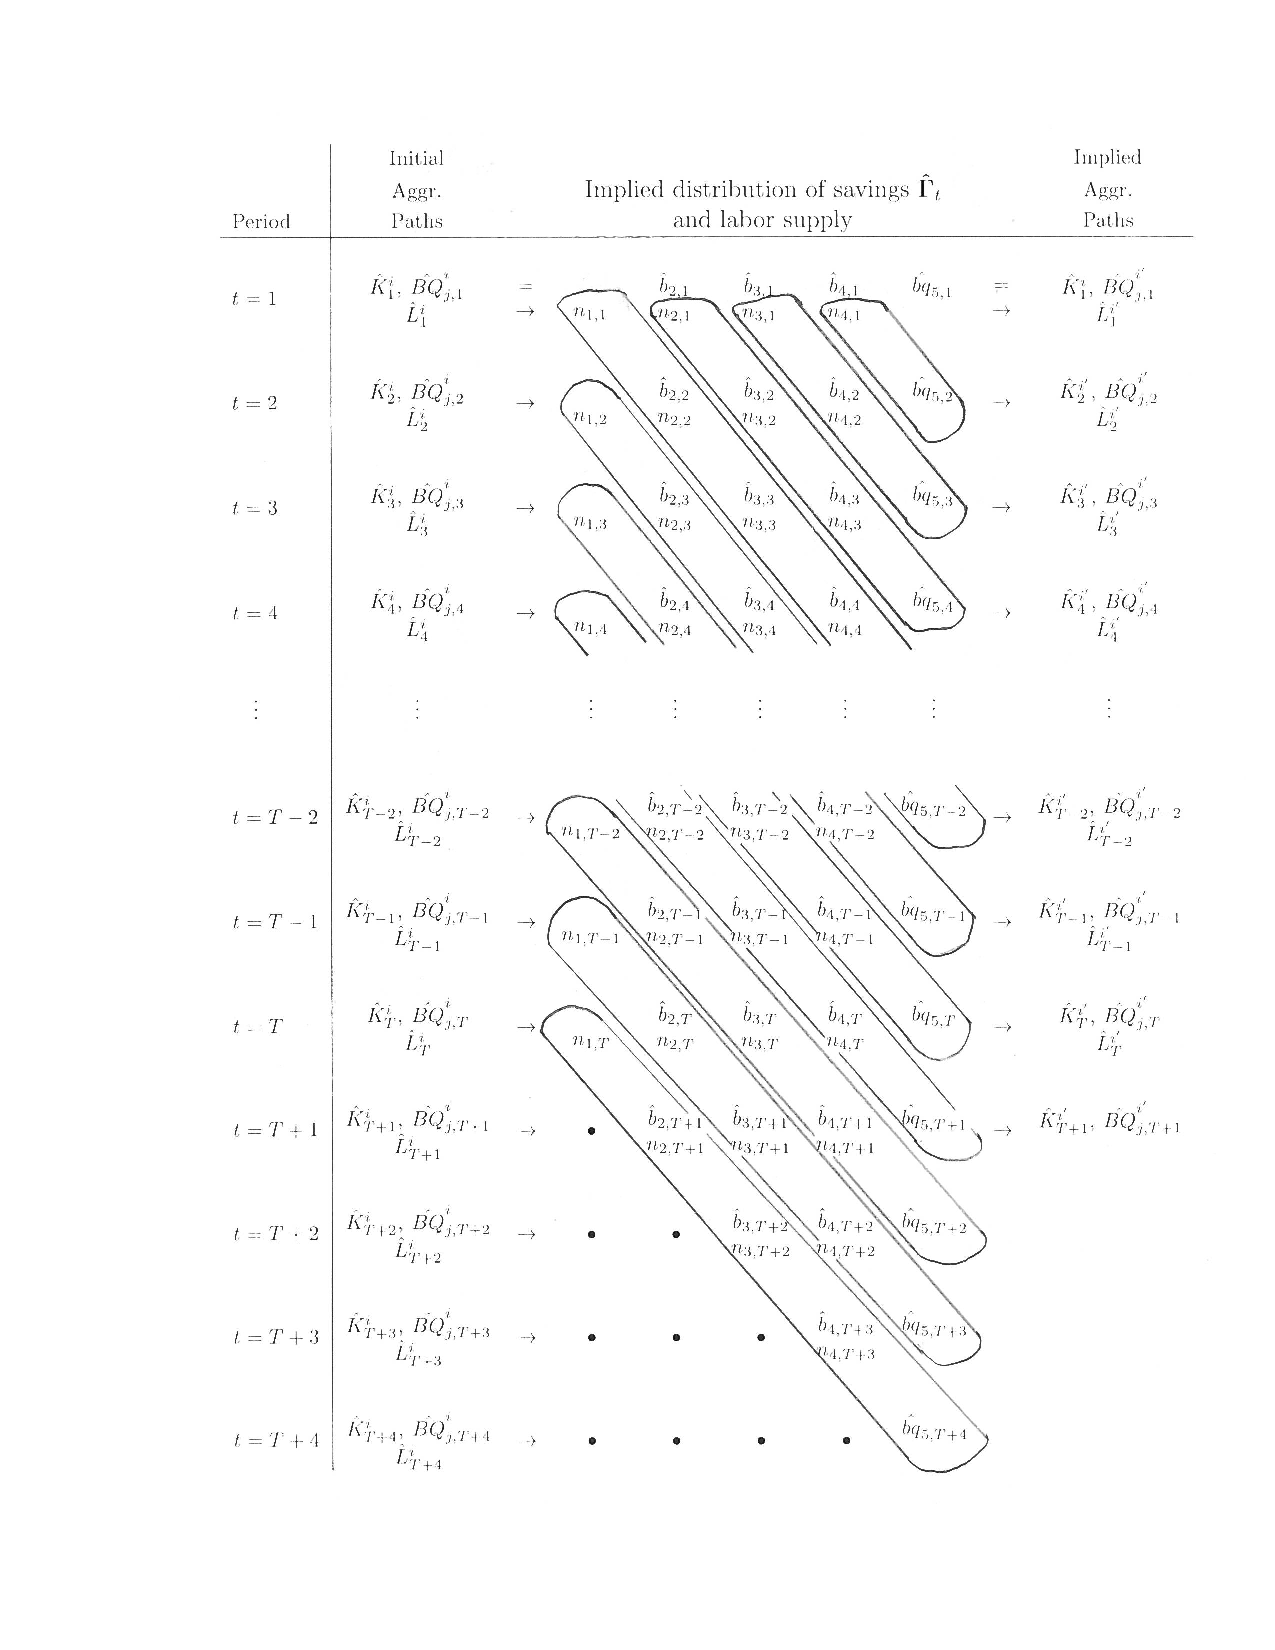
\includegraphics{images/TPIdiag.pdf}}}
  \end{figure}


  % THIS IS THE CODE FOR THE TABLE UNDERLYING THE FIGURE ABOVE
  % \begin{tabular}{>{\footnotesize}l| >{\footnotesize}c >{\footnotesize}c >{\footnotesize}c >{\footnotesize}c >{\footnotesize}c >{\footnotesize}c >{\footnotesize}c >{\footnotesize}c >{\footnotesize}c}
  %          & Initial & & & & & & & & Implied \\
  %          & Aggr. & & \multicolumn{5}{c}{Implied distribution of savings $\bm{\hat{\Gamma}}_t$} & & Aggr. \\
  %   Period & Paths    & & \multicolumn{5}{c}{and labor supply}   & & Paths    \\
  %   \hline
  %   & & & & & & & & & \\
  %   $t=1$ & $\begin{matrix}\hat{K}_1^i, \: \hat{BQ}_{j,1}^i \\ \hat{L}_1^i\end{matrix}$ & $\begin{matrix}= \\ \rightarrow\end{matrix}$ & $\begin{matrix}\: \\ n_{1,1}\end{matrix}$ & $\begin{matrix}\hat{b}_{2,1} \\ n_{2,1}\end{matrix}$ & $\begin{matrix}\hat{b}_{3,1} \\ n_{3,1}\end{matrix}$ & $\begin{matrix}\hat{b}_{4,1} \\ n_{4,1}\end{matrix}$ & $\begin{matrix}\hat{bq}_{5,1} \\ \,\end{matrix}$ & $\begin{matrix}= \\ \rightarrow\end{matrix}$ & $\begin{matrix}\hat{K}_1^i, \: \hat{BQ}_{j,1}^{i'} \\ \hat{L}^{i'}_1\end{matrix}$ \\[10mm]
  %   $t=2$ & $\begin{matrix}\hat{K}_2^i, \: \hat{BQ}_{j,2}^i \\ \hat{L}^i_2\end{matrix}$ & $\rightarrow$ & $\begin{matrix}\: \\ n_{1,2}\end{matrix}$ & $\begin{matrix}\hat{b}_{2,2} \\ n_{2,2}\end{matrix}$ & $\begin{matrix}\hat{b}_{3,2} \\ n_{3,2}\end{matrix}$ & $\begin{matrix}\hat{b}_{4,2} \\ n_{4,2}\end{matrix}$ & $\begin{matrix}\hat{bq}_{5,2} \\ \,\end{matrix}$ & $\rightarrow$ & $\begin{matrix}\hat{K}_2^{i'}, \: \hat{BQ}_{j,2}^{i'} \\ \hat{L}^{i'}_2\end{matrix}$ \\[10mm]
  %   $t=3$ & $\begin{matrix}\hat{K}_3^i, \: \hat{BQ}_{j,3}^i \\ \hat{L}^i_3\end{matrix}$ & $\rightarrow$ & $\begin{matrix}\: \\ n_{1,3}\end{matrix}$ & $\begin{matrix}\hat{b}_{2,3} \\ n_{2,3}\end{matrix}$ & $\begin{matrix}\hat{b}_{3,3} \\ n_{3,3}\end{matrix}$ & $\begin{matrix}\hat{b}_{4,3} \\ n_{4,3}\end{matrix}$ & $\begin{matrix}\hat{bq}_{5,3} \\ \,\end{matrix}$ & $\rightarrow$ & $\begin{matrix}\hat{K}_3^{i'}, \: \hat{BQ}_{j,3}^{i'} \\ \hat{L}^{i'}_3\end{matrix}$ \\[10mm]
  %   $t=4$ & $\begin{matrix}\hat{K}_4^i, \: \hat{BQ}_{j,4}^i \\ \hat{L}^i_4\end{matrix}$ & $\rightarrow$ & $\begin{matrix}\: \\ n_{1,4}\end{matrix}$ & $\begin{matrix}\hat{b}_{2,4} \\ n_{2,4}\end{matrix}$ & $\begin{matrix}\hat{b}_{3,4} \\ n_{3,4}\end{matrix}$ & $\begin{matrix}\hat{b}_{4,4} \\ n_{4,4}\end{matrix}$ & $\begin{matrix}\hat{bq}_{5,4} \\ \,\end{matrix}$ & $\rightarrow$ & $\begin{matrix}\hat{K}_4^{i'}, \: \hat{BQ}_{j,4}^{i'} \\ \hat{L}^{i'}_4\end{matrix}$ \\[10mm]
  %   $\quad\vdots$ & $\vdots$ & & $\vdots$ & $\vdots$ & $\vdots$ & $\vdots$ & $\vdots$ & & $\vdots$ \\[10mm]
  %   $t=T-2$ & $\begin{matrix}\hat{K}_{T-2}^i, \: \hat{BQ}_{j,T-2}^i \\ \hat{L}^i_{T-2}\end{matrix}$ & $\rightarrow$ & $\begin{matrix}\: \\ n_{1,T-2}\end{matrix}$ & $\begin{matrix}\hat{b}_{2,T-2} \\ n_{2,T-2}\end{matrix}$ & $\begin{matrix}\hat{b}_{3,T-2} \\ n_{3,T-2}\end{matrix}$ & $\begin{matrix}\hat{b}_{4,T-2} \\ n_{4,T-2}\end{matrix}$ & $\begin{matrix}\hat{bq}_{5,T-2} \\ \,\end{matrix}$ & $\rightarrow$ & $\begin{matrix}\hat{K}_{T-2}^{i'}, \: \hat{BQ}_{j,T-2}^{i'} \\ \hat{L}^{i'}_{T-2}\end{matrix}$ \\[10mm]
  %   $t=T-1$ & $\begin{matrix}\hat{K}_{T-1}^i, \: \hat{BQ}_{j,T-1}^i \\ \hat{L}^i_{T-1}\end{matrix}$ & $\rightarrow$ & $\begin{matrix}\: \\ n_{1,T-1}\end{matrix}$ & $\begin{matrix}\hat{b}_{2,T-1} \\ n_{2,T-1}\end{matrix}$ & $\begin{matrix}\hat{b}_{3,T-1} \\ n_{3,T-1}\end{matrix}$ & $\begin{matrix}\hat{b}_{4,T-1} \\ n_{4,T-1}\end{matrix}$ & $\begin{matrix}\hat{bq}_{5,T-1} \\ \,\end{matrix}$ & $\rightarrow$ & $\begin{matrix}\hat{K}_{T-1}^{i'}, \: \hat{BQ}_{j,T-1}^{i'} \\ \hat{L}^{i'}_{T-1}\end{matrix}$ \\[10mm]
  %   $t=T$ & $\begin{matrix}\hat{K}_{T}^i, \: \hat{BQ}_{j,T}^i \\ \hat{L}^i_{T}\end{matrix}$ & $\rightarrow$ & $\begin{matrix}\: \\ n_{1,T}\end{matrix}$ & $\begin{matrix}\hat{b}_{2,T} \\ n_{2,T}\end{matrix}$ & $\begin{matrix}\hat{b}_{3,T} \\ n_{3,T}\end{matrix}$ & $\begin{matrix}\hat{b}_{4,T} \\ n_{4,T}\end{matrix}$ & $\begin{matrix}\hat{bq}_{5,T} \\ \,\end{matrix}$ & $\rightarrow$ & $\begin{matrix}\hat{K}_{T}^{i'}, \: \hat{BQ}_{j,T}^{i'} \\ \hat{L}^{i'}_{T}\end{matrix}$ \\[10mm]
  %   $t=T+1$ & $\begin{matrix}\hat{K}_{T+1}^i, \: \hat{BQ}_{j,T+1}^i \\ \hat{L}^i_{T+1}\end{matrix}$ & $\rightarrow$ & $\bullet$ & $\begin{matrix}\hat{b}_{2,T+1} \\ n_{2,T+1}\end{matrix}$ & $\begin{matrix}\hat{b}_{3,T+1} \\ n_{3,T+1}\end{matrix}$ & $\begin{matrix}\hat{b}_{4,T+1} \\ n_{4,T+1}\end{matrix}$ & $\begin{matrix}\hat{bq}_{5,T+1} \\ \,\end{matrix}$ & $\rightarrow$ & $\begin{matrix}\hat{K}_{T+1}^{i'}, \: \hat{BQ}_{j,T+1}^{i'} \\ \:\end{matrix}$ \\[10mm]
  %   $t=T+2$ & $\begin{matrix}\hat{K}_{T+2}^i, \: \hat{BQ}_{j,T+2}^i \\ \hat{L}^i_{T+2}\end{matrix}$ & $\rightarrow$ & $\bullet$ & $\bullet$ & $\begin{matrix}\hat{b}_{3,T+2} \\ n_{3,T+2}\end{matrix}$ & $\begin{matrix}\hat{b}_{4,T+2} \\ n_{4,T+2}\end{matrix}$ & $\begin{matrix}\hat{bq}_{5,T+2} \\ \,\end{matrix}$ & & \\[10mm]
  %   $t=T+3$ & $\begin{matrix}\hat{K}_{T+3}^i, \: \hat{BQ}_{j,T+3}^i \\ \hat{L}^i_{T+3}\end{matrix}$ & $\rightarrow$ & $\bullet$ & $\bullet$ & $\bullet$ & $\begin{matrix}\hat{b}_{4,T+3} \\ n_{4,T+3}\end{matrix}$ & $\begin{matrix}\hat{bq}_{5,T+3} \\ \,\end{matrix}$ & & \\[10mm]
  %   $t=T+4$ & $\begin{matrix}\hat{K}_{T+4}^i, \: \hat{BQ}_{j,T+4}^i \\ \hat{L}^i_{T+4}\end{matrix}$ & $\rightarrow$ & $\bullet$ & $\bullet$ & $\bullet$ & $\bullet$ & $\begin{matrix}\hat{bq}_{5,T+4} \\ \,\end{matrix}$ & & \\
  % \end{tabular}
  % \clearpage

  Once the set of lifetime saving and labor supply decisions has been computed for all individuals alive in $1\leq t\leq T$, we use the individual decisions to compute a new implied time path of the aggregate capital stock and aggregate labor. The implied paths of the aggregate capital stock $\bm{\hat{K}}^{i'}=\{\hat{K}_1^i,\hat{K}_2^{i'},...\hat{K}_T^{i'}\}$, aggregate labor $\bm{\hat{L}}^{i'}=\{\hat{L}_1^i,\hat{L}_2^{i'},...\hat{L}_T^{i'}\}$, and total bequests received $\bm{\hat{BQ}}_j^{i'}=\{\hat{BQ}_{j,1}^i,\hat{BQ}_{j,2}^{i'},...\hat{BQ}_{j,T}^{i'}\}$ in general do not equal the initial guessed paths $\bm{\hat{K}}^{i}=\{\hat{K}_1^i,\hat{K}_2^{i},...\hat{K}_T^{i}\}$, $\bm{\hat{L}}^{i}=\{\hat{L}_1^i,\hat{L}_2^{i},...\hat{L}_T^{i}\}$, and $\bm{\hat{BQ}}_j^{i}=\{\hat{BQ}_{j,1}^i,\hat{BQ}_{j,2}^{i},...\hat{BQ}_{j,T}^{i}\}$ used to compute the individual savings and labor supply decisions $\bm{\hat{K}}^{i'}\neq\bm{\hat{K}}^i$, $\bm{\hat{L}}^{i'}\neq\bm{\hat{L}}^i$, and $\bm{\hat{BQ}}_j^{i'}\neq\bm{\hat{BQ}}_j^i$.

  Let $\norm{\:\cdot\:}$ be a norm on the space of time paths of the aggregate capital stock $\bm{\hat{K}}\in\mathcal{K}\subset\mathbb{R}_{++}^T$, aggregate labor supply $\bm{\hat{L}}\in\mathcal{L}\subset\mathbb{R}_{++}^T$, and $J$ paths of total bequests received $\bm{\hat{BQ}}_j\in\mathcal{B}\subset\mathbb{R}_{++}^T$. Then the fixed point necessary for the equilibrium transition path from Definition \ref{DefEquilNonSS} has been found when the distance between these $J+2$ paths is arbitrarily close to zero.
  \begin{equation}\label{EqTPIconverge}
    \norm{\Bigl[\bm{\hat{K}}^{i'}, \bm{\hat{L}}^{i'},\bigl\{\bm{\hat{BQ}}_j^{i'}\bigr\}_{j=1}^J\Bigr] - \Bigl[\bm{\hat{K}}^{i},\bm{\hat{L}}^{i},\bigl\{\bm{\hat{BQ}}_j^{i}\bigr\}_{j=1}^J\Bigr]} \leq \ve \quad\text{for}\quad \ve>0
  \end{equation}
  If the fixed point has not been found $\norm{\Bigl[\bm{\hat{K}}^{i'}, \bm{\hat{L}}^{i'},\bigl\{\bm{\hat{BQ}}_j^{i'}\bigr\}_{j=1}^J\Bigr] - \Bigl[\bm{\hat{K}}^{i},\bm{\hat{L}}^{i},\bigl\{\bm{\hat{BQ}}_j^{i}\bigr\}_{j=1}^J\Bigr]} > \ve$, then new transition paths for the aggregate capital stock and aggregate labor are generated as a convex combination of $\Bigl[\bm{\hat{K}}^{i'},\bm{\hat{L}}^{i'},\bigl\{\bm{\hat{BQ}}_j^{i'}\bigr\}_{j=1}^J\Bigr]$ and $\Bigl[\bm{\hat{K}}^{i},\bm{\hat{L}}^{i},\bigl\{\bm{\hat{BQ}}_j^{i}\bigr\}_{j=1}^J\Bigr]$.
  \begin{equation}\label{EqTPInewpath}
    \begin{split}
      \bm{\hat{K}}^{i+1} &= \nu\bm{\hat{K}}^{i'} + (1-\nu)\bm{\hat{K}}^{i} \\
      \bm{\hat{L}}^{i+1} &= \nu\bm{\hat{L}}^{i'} + (1-\nu)\bm{\hat{L}}^{i} \\
      \bm{\hat{BQ}}_1^{i+1} &= \nu\bm{\hat{BQ}}_1^{i'} + (1-\nu)\bm{\hat{BQ}}_1^{i} \\
      &\vdots \\
      \bm{\hat{BQ}}_J^{i+1} &= \nu\bm{\hat{BQ}}_J^{i'} + (1-\nu)\bm{\hat{BQ}}_J^{i}
    \end{split} \quad\quad\text{for}\quad \nu\in(0,1]
  \end{equation}
  This process is repeated until the initial transition paths for the aggregate capital stock, aggregate labor, and total bequests received are consistent with the transition paths implied by those beliefs and individual and firm optimization.

  In essence, the TPI method iterates on individual beliefs about the time path of prices represented by a time paths for the aggregate capital stock $\bm{\hat{K}}^i$, aggregate labor $\bm{\hat{L}}^i$, and total bequests received $\bm{\hat{BQ}}_j^i$ until a fixed point in beliefs is found that are consistent with the transition paths implied by optimization based on those beliefs.

  The following are the steps for computing a stationary non-steady-state equilibrium time path for the economy.
  \begin{enumerate}
    \item Input all initial parameters. See Table \ref{TabExogVars}.
      \begin{enumerate}
        \item The value for $T$ at which the non-steady-state transition path should have converged to the steady state should be at least as large as the number of periods it takes the population to reach its steady state $\bm{\bar{\omega}}$ as described in Appendix \ref{AppPopGrowth}.
      \end{enumerate}

    \item Choose an initial distribution of savings and intended bequests $\bm{\hat{\Gamma}}_1$ and then calculat the initial state of the stationarized aggregate capital stock $\hat{K}_1$ and total bequests received $\hat{BQ}_{j,1}$ consistent with $\bm{\hat{\Gamma}}_1$ according to \eqref{EqMktClrCapStat} and \eqref{EqTotBeqStat1}.
      \begin{enumerate}
        \item Note that you must have the population weights from the previous period $\hat{\omega}_{s,0}$ and the growth rate between period 0 and period 1 $\tilde{g}_{n,1}$to calculate $\hat{BQ}_{j,1}$.
      \end{enumerate}
    \item Conjecture transition paths for the stationarized aggregate capital stock $\bm{\hat{K}}^1=\{\hat{K}^1_t\}_{t=1}^\infty$, stationarized aggregate labor $\bm{\hat{L}}^1=\{\hat{L}^1_t\}_{t=1}^\infty$, and total bequests received $\bm{\hat{BQ}}_j^1=\{\hat{BQ}^{1}_{j,t}\}_{t=1}^\infty$ where the only requirements are that $\hat{K}^i_1$ and $\hat{BQ}^i_{j,1}$ are functions of the initial distribution of savings $\bm{\hat{\Gamma}}_1$ for all $i$ is your initial state and that $\hat{K}^i_t=\bar{K}$, $\hat{L}^i_t=\bar{L}$, and $\hat{BQ}^i_{j,t}= \bar{BQ}_j$ for all $t\geq T$. The conjectured transition paths of the aggregate capital stock $\bm{\hat{K}}^i$ and aggregate labor $\bm{\hat{L}}^i$ imply specific transition paths for the real wage $\bm{\hat{w}}^i=\{\hat{w}^i_t\}_{t=1}^\infty$ and the real interest rate $\bm{r}^i=\{r^i_t\}_{t=1}^\infty$ through expressions \eqref{EqFOCwageStat} and \eqref{EqFOCrate}.
      \begin{enumerate}
        \item An intuitive choice for the time path of aggregate labor is the steady-state in every period $\hat{L}^1_t = \bar{L}$ for all $t$.
      \end{enumerate}
    \item With the conjectured transition paths $\bm{\hat{w}}^i$, $\bm{r}^i$, and $\bm{\hat{BQ}}_j^i$ one can solve for the lifetime policy functions of each individual alive at time $1\leq t\leq T$ using the systems of Euler equations of the form \eqref{EqEulerLabStat}, \eqref{EqEulerSavStat}, and \eqref{EqEulerSavEpSstat} and following the diagram in Figure \ref{FigTPIdiag}.
    \item Use the implied distribution of savings and labor supply in each period (each row of $\hat{b}_{j,s,t}$ and $n_{j,s,t}$ in Figure \ref{FigTPIdiag}) to compute the new implied time paths for the aggregate capital stock $\bm{\hat{K}}^{i'} = \{\hat{K}_1^i,\hat{K}_2^{i'},...\hat{K}_T^{i'}\}$, aggregate labor supply $\bm{\hat{L}}^{i'} = \{\hat{L}_1^i,\hat{L}_2^{i'},...\hat{L}_T^{i'}\}$, and total bequests received $\bm{\hat{BQ}}_j^{i'} = \{\hat{BQ}_{j,1}^i,\hat{BQ}_{j,2}^{i'},...\hat{BQ}_{j,T}^{i'}\}$.
    \item Check the distance between the two sets time paths.
      \begin{equation*}
        \norm{\Bigl[\bm{\hat{K}}^{i'}, \bm{\hat{L}}^{i'},\bigl\{\bm{\hat{BQ}}_j^{i'}\bigr\}_{j=1}^J\Bigr] - \Bigl[\bm{\hat{K}}^{i},\bm{\hat{L}}^{i},\bigl\{\bm{\hat{BQ}}_j^{i}\bigr\}_{j=1}^J\Bigr]}
      \end{equation*}
      \begin{enumerate}
        \item If the distance between the initial time paths and the implied time paths is less-than-or-equal-to some convergence criterion $\ve>0$, then the fixed point has been achieved and the equilibrium time path has been found \eqref{EqTPIconverge}.
        \item If the distance between the initial time paths and the implied time paths is greater than some convergence criterion $\norm{\cdot}>\ve$, then update the guess for the time paths according to \eqref{EqTPInewpath} and repeat steps (4) through (6) until a fixed point is reached.
      \end{enumerate}
  \end{enumerate}

  \clearpage


\end{document}
